\documentclass[11pt]{article}
\usepackage[margin=1in]{geometry}
\usepackage[T1]{fontenc}
\usepackage[utf8]{inputenc}
\usepackage{lmodern}
\usepackage{booktabs}
\usepackage{array}
\usepackage{colortbl}
% Booktabs leaves rows unruled on purpose, which reads well when every cell is one line.
% These tables have cells that wrap to three lines, and without a separator the eye loses
% which fragment belongs to which row. A hairline in light grey is enough to hold the row
% together without turning the table into a grid.
\newcommand{\rowrule}{\arrayrulecolor{black!22}\midrule\arrayrulecolor{black}}
\renewcommand{\arraystretch}{1.18}
\usepackage{enumitem}
\usepackage{rotating}
\usepackage{hyperref}
\usepackage{xcolor}
\usepackage{tikz}
\usepackage{graphicx}
\usepackage{amsmath}
\usetikzlibrary{arrows.meta,positioning,shapes.misc,backgrounds}
\hypersetup{colorlinks=true,linkcolor=blue!50!black,urlcolor=blue!50!black}
\setlist{nosep}
\definecolor{claude}{HTML}{7A55CC}
\definecolor{jev}{HTML}{2E9E63}
\definecolor{code}{HTML}{3A7BC0}

\title{Jezero Ops: splitting a rover's mind between a System One and a System Two}
\author{Kevin Horton\\\small built with Claude Code, TypeSafe's \emph{jev}, three.js, Blender, and NASA/USGS data}
\date{September 2026}

\begin{document}
\maketitle

\begin{center}\fbox{\parbox{0.92\textwidth}{\small\textbf{This is a demo.} Not flight software, not a research result, and not validated against any real rover. It exists to make one idea visible: that a robot's decisions split into two kinds, and that two very different models can take the two kinds.}}\end{center}

\begin{abstract}
A Mars rover has two kinds of thinking to do: slow, deliberate, argued-from-evidence planning and interpretation, and fast, narrow, high-frequency judgment. JPL splits these between a ground team and onboard flight software. We split them between two very different AI systems and made the split visible on screen. \textcolor{claude}{\textbf{Claude}}, a large language model, plays the science team and tactical planners. \textcolor{jev}{\textbf{jev}}, TypeSafe's System One model, plays the onboard judgment, returning typed answers with calibrated probabilities in about 250\,ms. \textcolor{code}{\textbf{Code}} owns everything that should never be a judgment call: geometry, budgets, thresholds, and the state machine. The result is a playable, recorded simulation of Perseverance on real USGS Jezero terrain, in which every decision is attributed to the engine that made it. It was built twice in one day: first as a browser prototype (HTML, CSS and three.js with a small Node server), then moved onto ROS\,2 Jazzy, where the browser became only the simulator and every decision became a node with a typed interface. All screenshots in this report are from the ROS\,2 run. In a later pass jev also became a tool \emph{inside} Claude's reasoning, so that part of the slow mind's work is done by fast judgment. The graph is flight-like: Claude calls are ROS\,2 actions with feedback and cancel, the executive is a behaviour tree, and jev reads every telemetry sample. The final pass stopped asserting and started measuring, and found two defects that qualitative description had hidden: a shadow-dropout model that tore shadowed boulders into fragments and reported them as flat shadows, and an arm collision model that under-estimated the turret by a factor of seven, letting it be driven into a rock while reporting clearance. Both are fixed and the fixes are quantified. The measurements also set the science stand-off, which had been chosen rather than derived. In the recorded run jev answered about 2\,900 typed questions across 760 calls for \$0.03, against \$1.10 for 13 Claude calls --- the economic argument for the split, in two numbers.
\end{abstract}

\section{Why two models and not one}

The obvious build is to put an LLM in the loop for everything. It fails in two directions at once. An LLM is too slow and too expensive to answer \emph{is that a rock?} every few metres, and it is not designed to return a \emph{calibrated probability}: asked whether something is a hazard it produces prose, not a number one can threshold. A System One model is the opposite. It does not reason, plan, or generate text. It is handed structured state and a set of narrow, typed questions --- a \textbf{Choice} over defined options, a yes/no \textbf{Noul}, a \textbf{Score} on ordered levels --- and returns a probability distribution over the answers in one fast call, together with a confidence that code can gate on. That is the shape of an onboard decision, and it is precisely \emph{not} the shape of ``write me a sol plan.''

The architecture therefore follows one rule twice, at two speeds: \emph{code owns the workflow; a model answers narrow typed questions.}

\begin{table}[h]
\centering\small
\begin{tabular}{@{}p{2.2cm}p{4.2cm}p{4.2cm}p{3.6cm}@{}}
\toprule
 & \textcolor{claude}{\textbf{CLAUDE} (System Two)} & \textcolor{jev}{\textbf{JEV} (System One)} & \textcolor{code}{\textbf{CODE}} \\
\midrule
Role & science team and rover planners & onboard judgment & flight rules, geometry, budgets \\
\rowrule
Input & everything: downlink, targets, hypotheses, history, Navcam frames & a filtered JSON state and typed questions & numbers \\
\rowrule
Output & plan / interpretation / report against a JSON schema & a probability per option, plus confidence & deterministic \\
\rowrule
Latency & 15--125\,s & about 250\,ms & microseconds \\
\rowrule
Called & a few times per sol & at every decision point & continuously \\
\rowrule
Never asked to & pick an arc, classify a blob & plan, reason, generate text, do arithmetic & judge anything semantic \\
\bottomrule
\end{tabular}
\caption{Division of labour.}
\end{table}

\section{The system}

\subsection{Built twice: browser first, then ROS\,2}
The first build was a web page: HTML and CSS for the HUD, the swimlane and the ops console, three.js for the terrain and the rover, and a Node server that held the two model calls. That prototype is where every decision path was designed and recorded once. It was then moved onto ROS\,2 (Section~\ref{sec:ros2}): the same browser page kept only what a simulator owns --- terrain, motion, cameras, rendering --- and talks to a graph of five nodes over rosbridge. The port changed no rule and no question; it changed where they live. The figures that follow are all from the ROS\,2 run, which is also why every screenshot carries the live ``ROS\,2 graph'' panel and the nine-camera rig in its corners.

\subsection{The world}
\begin{itemize}
\item \textbf{Terrain}: the USGS \emph{Mars 2020 Terrain Relative Navigation CTX DTM Mosaic} (20\,m/px) and its 6\,m/px orthomosaic, cropped to 1.28\,km around $18.4385^\circ$N, $77.4335^\circ$E --- the M\'aaz / S\'e\'itah / Artuby-ridge area Perseverance worked in its first year. The real 46\,m of relief drives the rover's pitch and roll and ENav's tilt checks \cite{fergason}.
\item \textbf{Rover}: the NASA/JPL-Caltech Perseverance 3D model \cite{nasa3d}; wheels separated in Blender so they roll, mast and arm animated.
\item \textbf{Synthetic, and labelled as such}: rover-scale micro-relief (fractal noise), a rock field from the Golombek cumulative-fractional-area model ($k=0.07$; $\approx 55\,000$ rocks $\ge 0.35$\,m in the central box) \cite{golombek}, each rock one of fourteen CC0 photogrammetry scans \cite{polyhaven} decimated to about 160 triangles, instanced and tinted to the M\'aaz/S\'e\'itah tones, a few ripple fields, and four scripted events so a twelve-minute run exercises every decision path.
\item \textbf{Targets} carry real names and simplified truth tables from published results: M\'aaz (basalt), Yeehgo, Rochette (the first cored rock; sulfate-filled fractures), Bastide at the S\'e\'itah contact (olivine cumulate altered to carbonate).
\end{itemize}

\subsection{The sol loop}
Claude is given JPL's tactical procedure as its own: assess downlink; choose science that discriminates between hypotheses; sequence remote sensing before contact science, abrasion before PIXL/SHERLOC, coring last; respect the envelope (900\,Wh, 300\,Mb, 420\,min, 200\,m) with 15\,\% margin; uplink \cite{jplplanning}. It returns a plan against a JSON schema: prioritised targets with instrument activities and rationale, a drive goal with constraints for the onboard system, a budget, and a plain-language \emph{criteria} string that is handed to jev for onboard target selection. Code lays the plan on a swimlane (one lane per subsystem, each instrument's Wh/min/Mb) and executes it block by block (Figures~\ref{fig:planning} and \ref{fig:science}).

\begin{figure}[p]
\centering
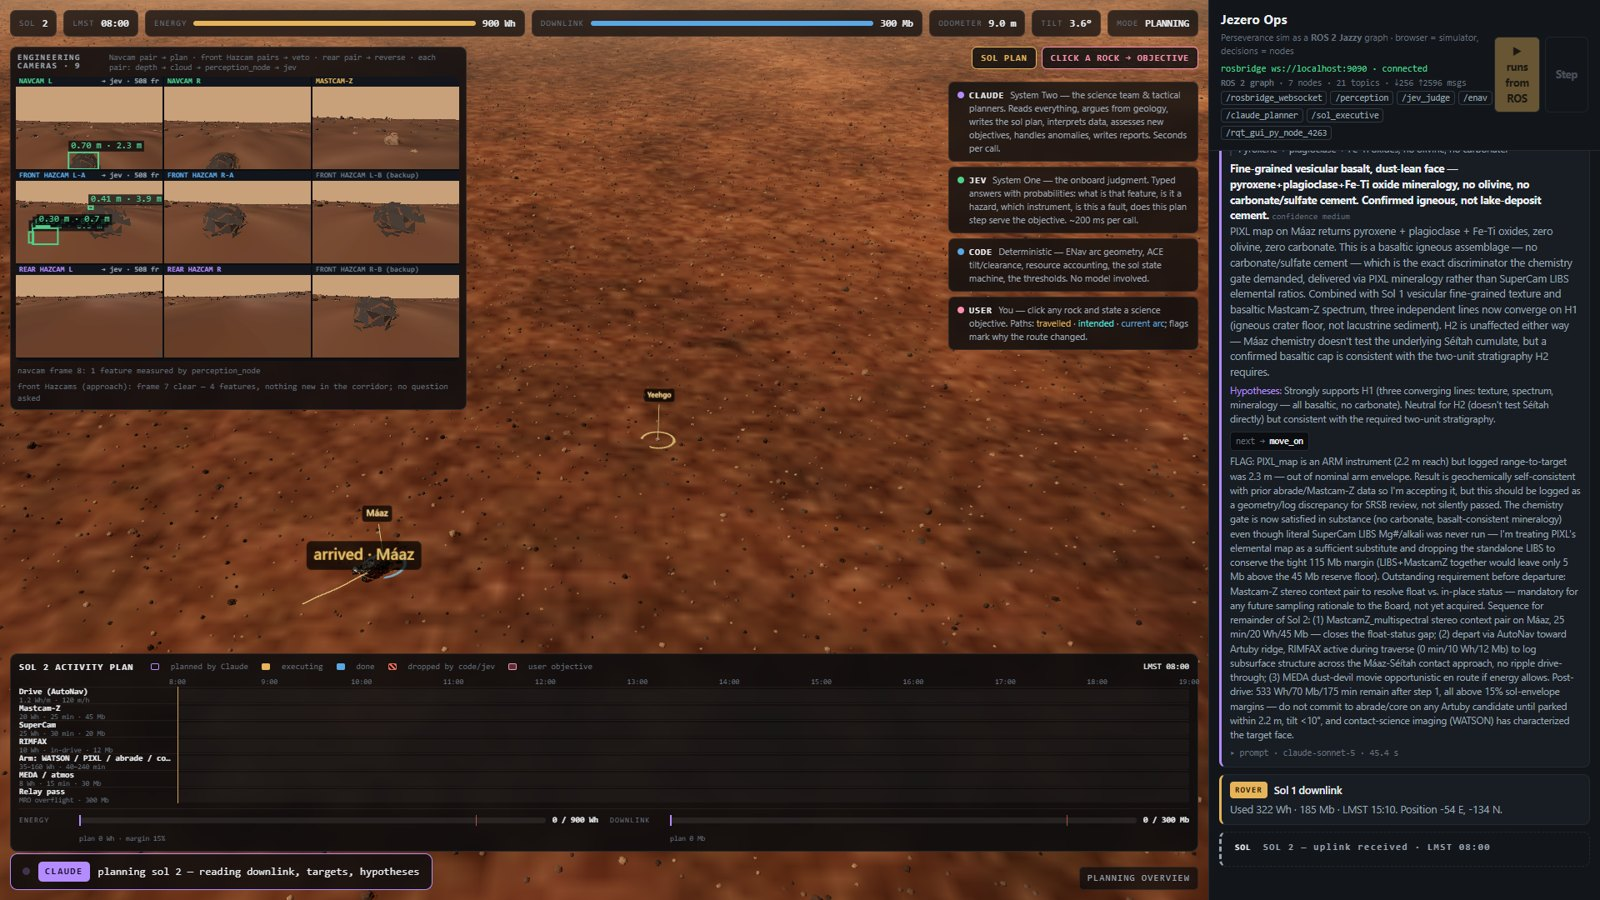
\includegraphics[width=\textwidth]{figs/planning-sol2.jpg}
\caption{Sol 2 planning, ROS\,2 run. Top: the HUD (sol, LMST, energy, downlink volume, odometer, tilt, mode). Top left: the nine-camera rig, idle at the parked rover. Bottom: the swimlane sol plan --- one lane per subsystem with each instrument's Wh, minutes and Mb, blocks coloured by state (planned by Claude, executing, done, dropped by code/jev, user objective) and the cumulative energy and data bars against the 15\,\% margin. Right: the console, every entry badged with the engine that produced it --- here Claude's PIXL interpretation from sol 1, the sol 1 downlink and the sol 2 uplink --- under the live graph panel (7 nodes, 21 topics, message counters).}
\label{fig:planning}
\end{figure}

\begin{figure}[p]
\centering
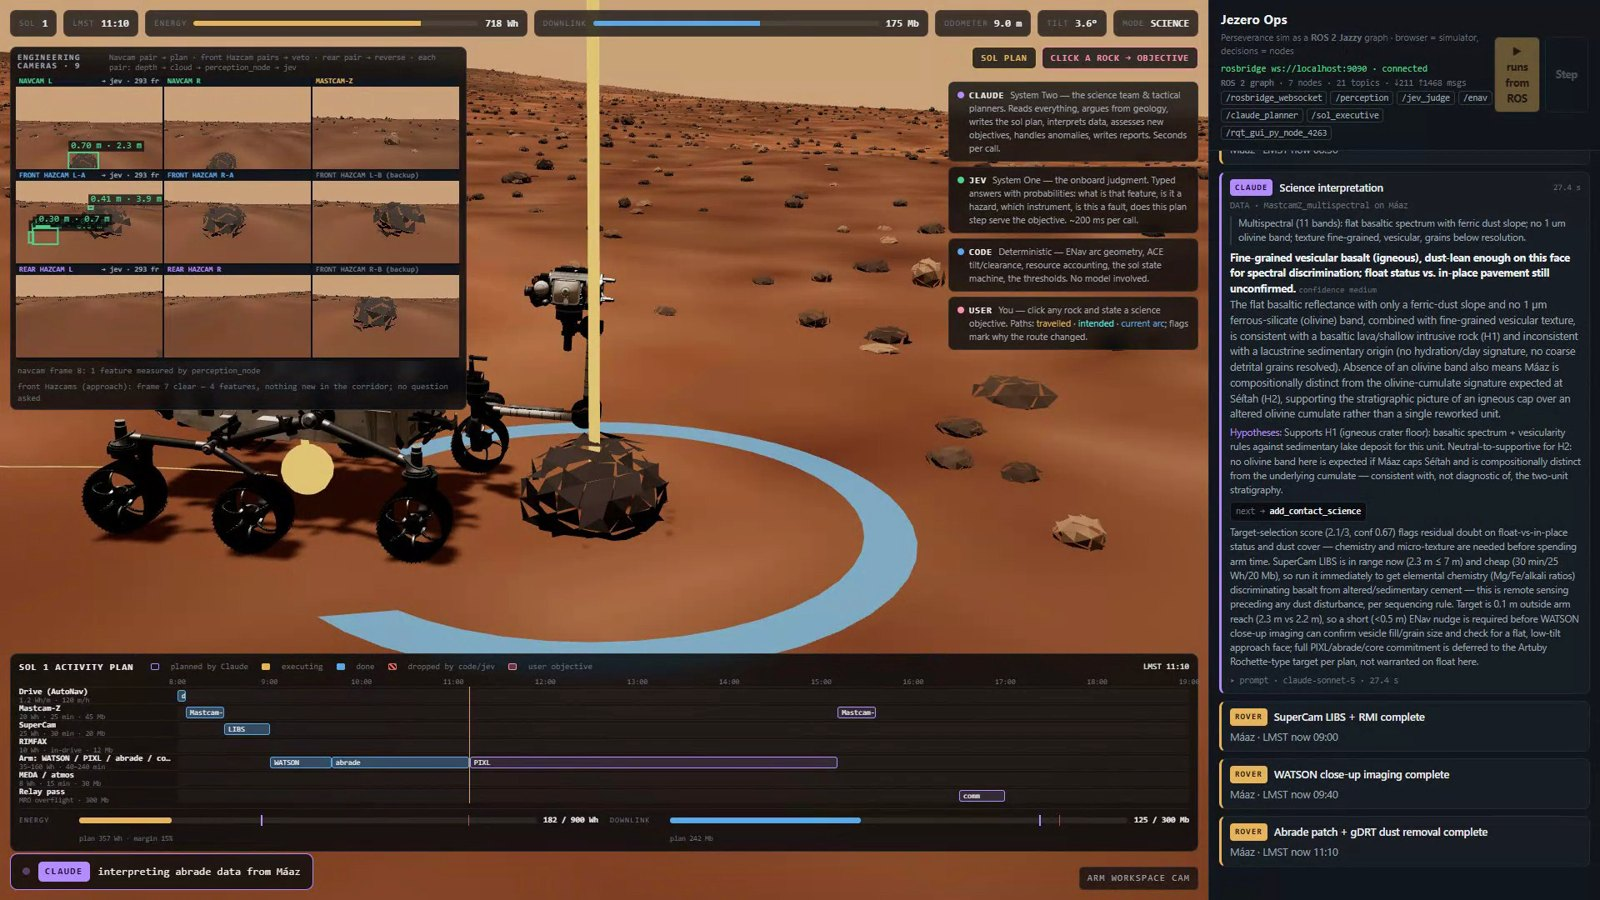
\includegraphics[width=\textwidth]{figs/science-maaz.jpg}
\caption{Contact science at Máaz, sol 1, from the arm-workspace camera (ROS\,2 run). The rig shows the Navcam pair with the target boxed at 2.3\,m and the front Hazcams with the two cobbles measured in the arm workspace. On the right, Claude's interpretation of the Mastcam-Z data (\emph{fine-grained vesicular basalt \ldots float status still unconfirmed}) and its next action --- LIBS first, then a short nudge into arm reach for WATSON --- followed by the activity completions; the swimlane shows WATSON, abrade and PIXL executing in the order the planners require.}
\label{fig:science}
\end{figure}

\subsection{Driving: perception, jev, ENav}

\begin{figure}[h]
\centering
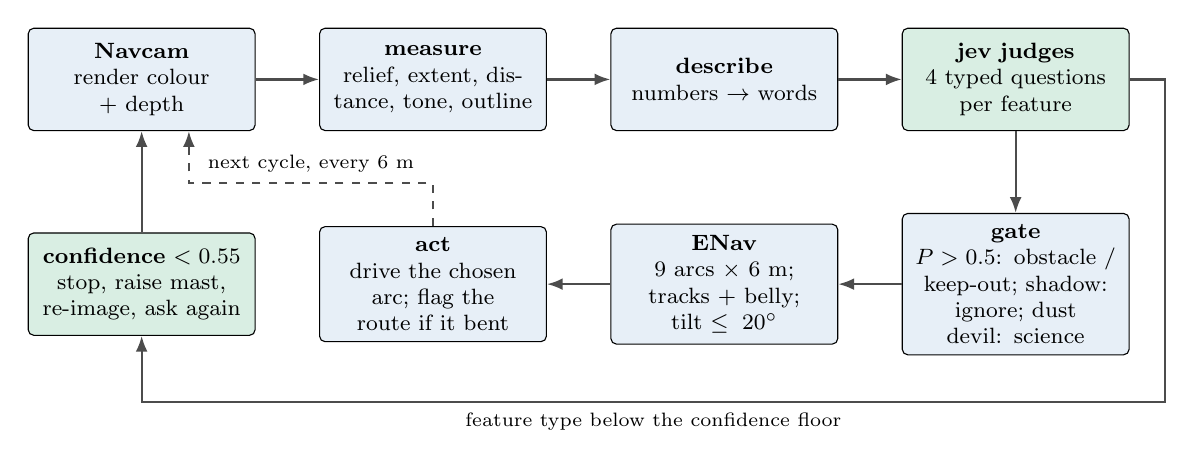
\begin{tikzpicture}[x=1cm, y=1cm, every node/.style={font=\footnotesize}, box/.style={draw, rounded corners=2pt, minimum height=13mm, inner sep=4pt, align=center, text width=26mm}, arr/.style={-{Latex[length=2mm]}, thick, draw=black!70}]
% row 1: perceive -> measure -> describe -> judge
\node[box, fill=code!12] (cam) at (0,0) {\textbf{Navcam}\\render colour + depth};
\node[box, fill=code!12] (blob) at (3.7,0) {\textbf{measure}\\relief, extent, distance, tone, outline};
\node[box, fill=code!12] (words) at (7.4,0) {\textbf{describe}\\numbers $\to$ words};
\node[box, fill=jev!18] (jev) at (11.1,0) {\textbf{jev judges}\\4 typed questions per feature};
% row 2: gate -> ENav -> act, and the confidence gate under the Navcam
\node[box, fill=code!12] (rules) at (11.1,-2.6) {\textbf{gate}\\$P>0.5$: obstacle / keep-out; shadow: ignore; dust devil: science};
\node[box, fill=code!12] (enav) at (7.4,-2.6) {\textbf{ENav}\\9 arcs $\times$ 6 m; tracks + belly; tilt $\le 20^\circ$};
\node[box, fill=code!12] (act) at (3.7,-2.6) {\textbf{act}\\drive the chosen arc; flag the route if it bent};
\node[box, fill=jev!18] (gate) at (0,-2.6) {\textbf{confidence $<0.55$}\\stop, raise mast, re-image, ask again};
\draw[arr] (cam) -- (blob); \draw[arr] (blob) -- (words); \draw[arr] (words) -- (jev);
\draw[arr] (jev) -- (rules); \draw[arr] (rules) -- (enav); \draw[arr] (enav) -- (act);
% low-confidence branch: around the bottom, into the confidence gate
\draw[arr] (jev.east) -- ++(0.45,0) |- (0,-4.1) node[pos=0.75, below, font=\scriptsize] {feature type below the confidence floor} -- (gate.south);
% gate -> Navcam (re-image), act -> Navcam (next cycle)
\draw[arr] (gate.north) -- (cam.south);
\draw[arr, dashed] (act.north) -- ++(0,0.55) -| node[pos=0.25, above, font=\scriptsize] {next cycle, every 6 m} ([xshift=6mm]cam.south);
\end{tikzpicture}
\caption{One imaging cycle while driving. Blue boxes are code, green are jev. Numbers are measured by code, turned into words, judged by jev as probabilities, and thresholded by code; the only way a model touches the drive is through a number a rule reads. Nothing here asks a model what to do next.}
\label{fig:cycle}
\end{figure}

The first version of the ``Navcam'' was a list lookup: rocks within a cone ahead were pulled from the world's rock table and described in words. It worked, but it was hard-coded knowledge dressed up as perception. In the final version the rover \emph{sees}. A camera rides the mast; each imaging cycle renders a colour frame and a depth frame (standing in for the stereo range map). Depth is unprojected to world points, relief above the local ground is measured, and connected blobs become features with the numbers a stereo pipeline produces: distance, bearing, extent, maximum relief, tone relative to the ground, outline, and how much of the blob is in shadow. Shadowed pixels are sampled sparsely, because real stereo fails in deep shadow --- which is what makes ``rock or shadow?'' a genuine question. In a probe against the world's truth table, rocks at 4--9\,m were located within 1--25\,cm and their relief measured within $\pm 3$\,cm.

Then the discipline that makes jev useful: \textbf{numbers become words before jev sees them}. jev is text-only by design (its documentation is explicit: pre-process images into text or structured fields) and it is weak at arithmetic, so code measures and jev judges. Four questions per feature, fanned out in one request:
\begin{itemize}
\item \texttt{feature\_type} --- Choice: embedded rock / loose rock / bedrock slab / sand ripples / shadow only / dust devil;
\item \texttt{wheel\_hazard} --- Noul: would a wheel over it risk damage or high-centring?
\item \texttt{sinkage\_risk} --- Noul: loose fine-grained material?
\item \texttt{science\_interest} --- Noul: worth an opportunistic observation?
\end{itemize}
Code applies the rules. A rock jev calls a wheel hazard, or that stereo measured above the 0.20\,m step limit, enters the \emph{perception map}; a ripple field with $P(\text{sinkage})>0.5$ becomes a 6\,m keep-out; a \texttt{shadow\_only} blob is ignored, where geometry alone would have stopped; a \texttt{dust\_devil} with $P(\text{science})>0.6$ schedules the MEDA/Navcam movie. And the \textbf{confidence gate}: if \texttt{feature\_type} returns with confidence below 0.55, code does not act on it --- the rover stops, raises the mast, takes a second stereo pair, and asks again.

ENav, the local planner, is pure code and plans only on what the rover has seen: nine candidate arcs, each checked for tilt and for rocks under the wheel tracks (step limit) or under the belly (clearance), plus jev's keep-outs \cite{enav}. The intended route is recomputed every cycle, so on screen it bends the moment a jev verdict lands, and a flag is planted on the track saying why and which engine caused it (Figures~\ref{fig:navcam}--\ref{fig:route}).

\begin{figure}[p]
\centering
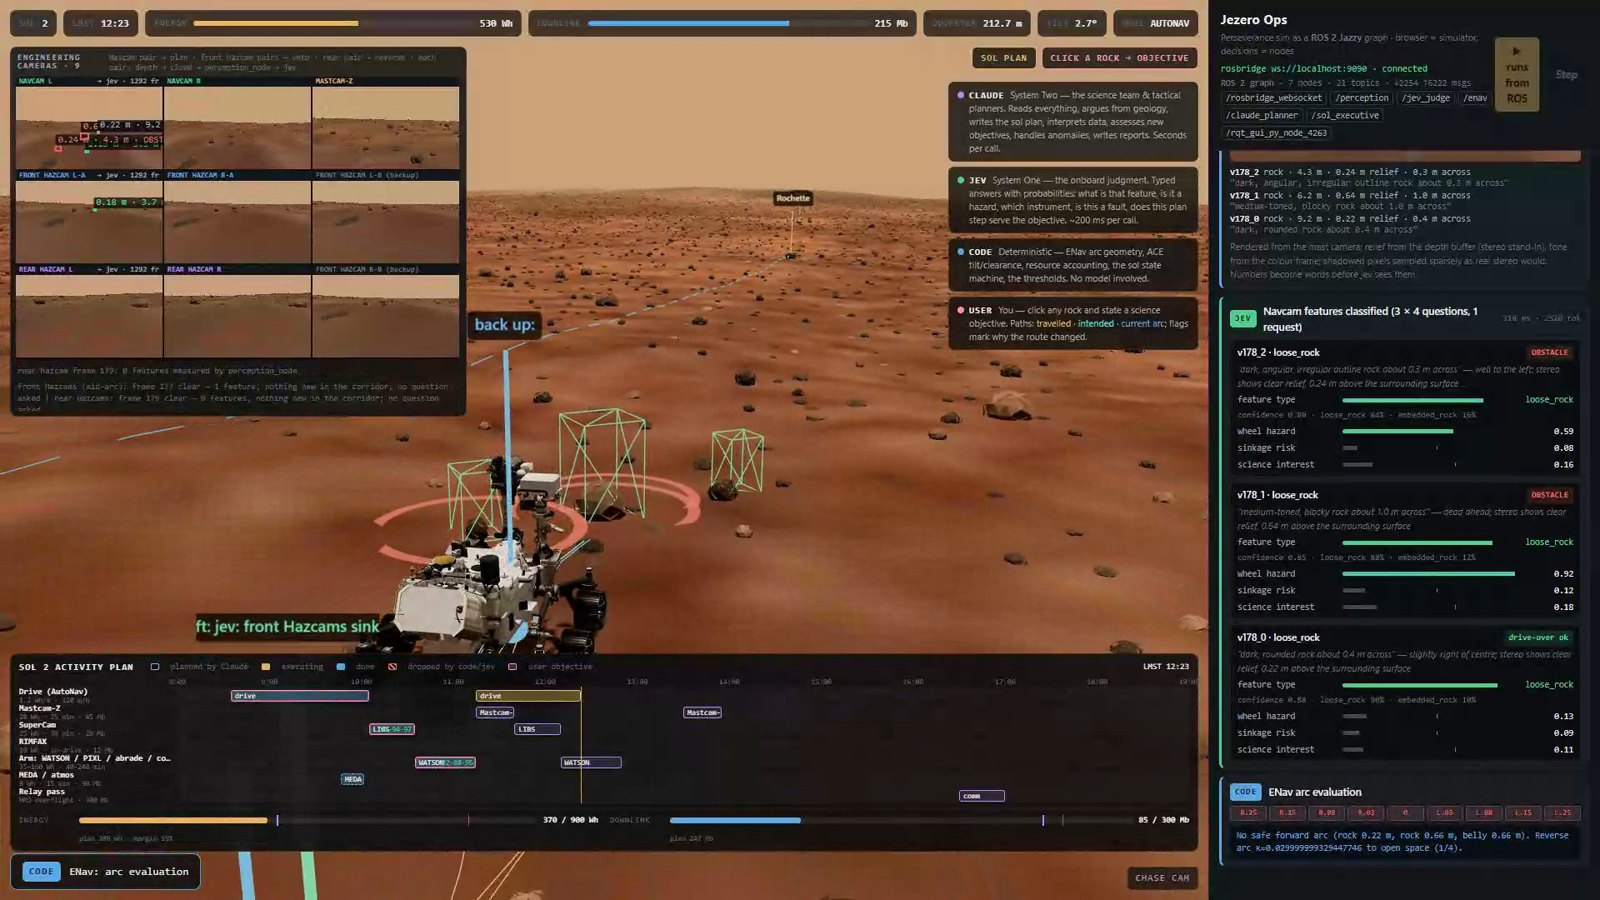
\includegraphics[width=\textwidth]{figs/navcam-obstacles.jpg}
\caption{A Navcam classification cycle on the sol-2 drive (ROS\,2 run). The Navcam L tile shows three measured rocks boxed with relief and range; the console shows the perception card (frame, numbers, words) and jev's answers: a 0.24\,m and a 0.64\,m rock become \textsc{obstacles} at $P(\text{wheel hazard})=0.59$ and $0.92$, a 0.22\,m rock is \emph{drive-over ok}. Wireframes mark the judged rocks; the red rings are earlier keep-outs. With the two obstacles in the perception map ENav finds no safe forward arc and backs out (``back up'' flag, reverse arc $\kappa=+0.03$). Twelve questions, one request, 318\,ms.}
\label{fig:navcam}
\end{figure}

\begin{figure}[p]
\centering
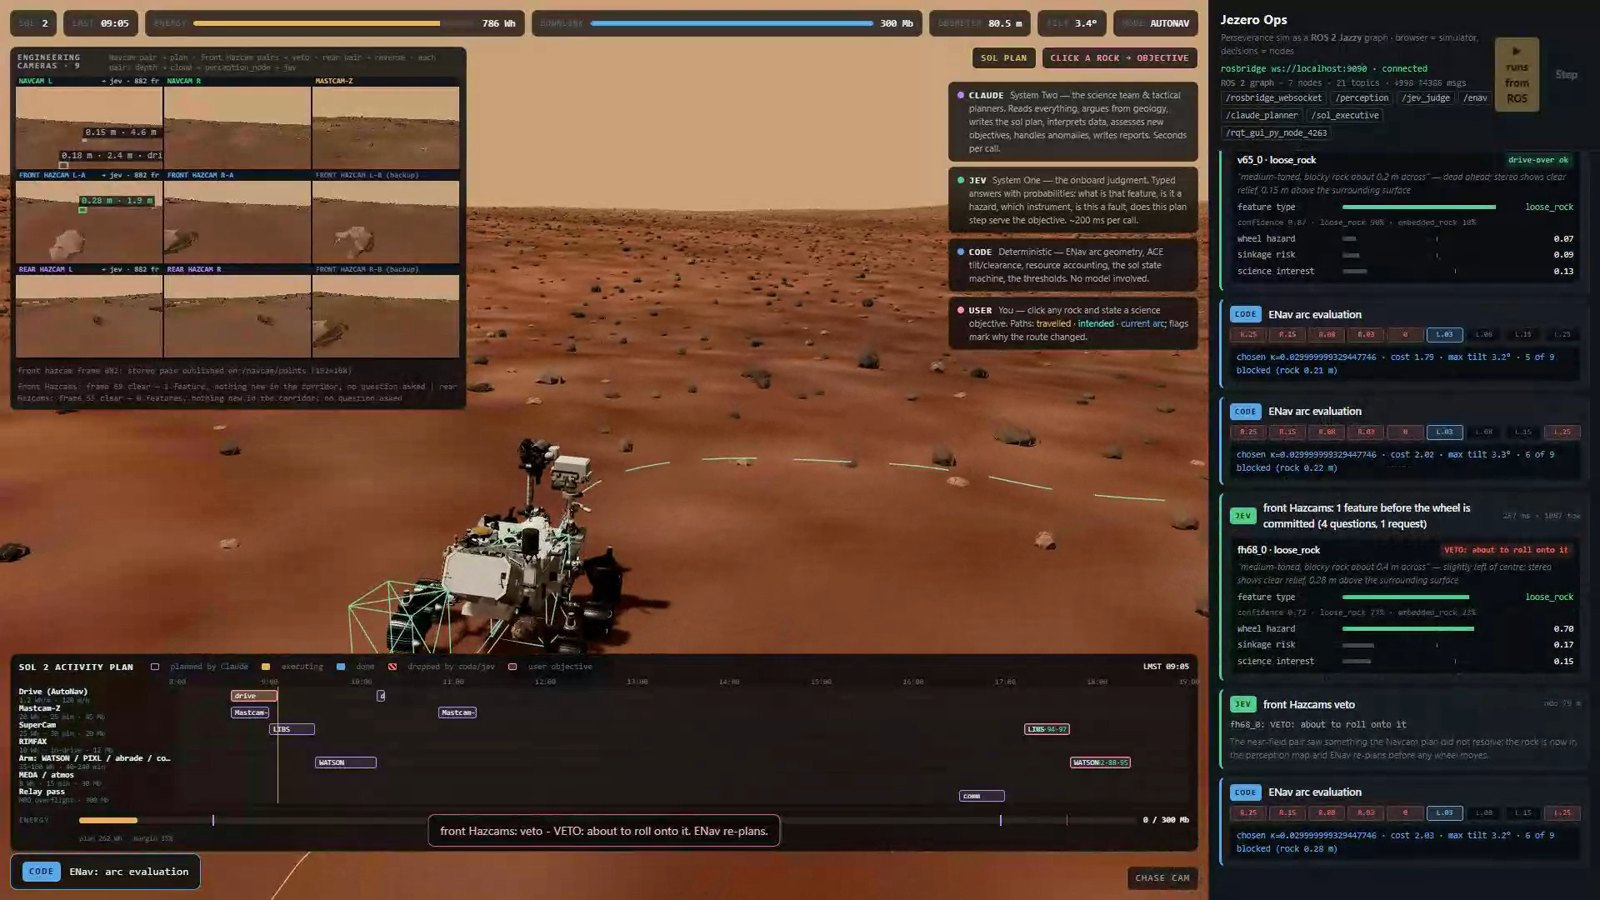
\includegraphics[width=\textwidth]{figs/hazcam-veto.jpg}
\caption{A front-Hazcam veto (ROS\,2 run). ENav had chosen an arc past a 0.28\,m rock the Navcam plan did not resolve; before the wheels were committed the front Hazcam pair measured it at 1.9\,m (tile, top left) and jev answered \emph{about to roll onto it} at $P=0.70$. The console shows the two ENav evaluations, the Hazcam card (one feature, four questions, one request), the \textsc{veto} entry, and ENav re-planning with the rock now in the perception map --- the wireframe beside the left front wheel.}
\label{fig:enav}
\end{figure}

\begin{figure}[p]
\centering
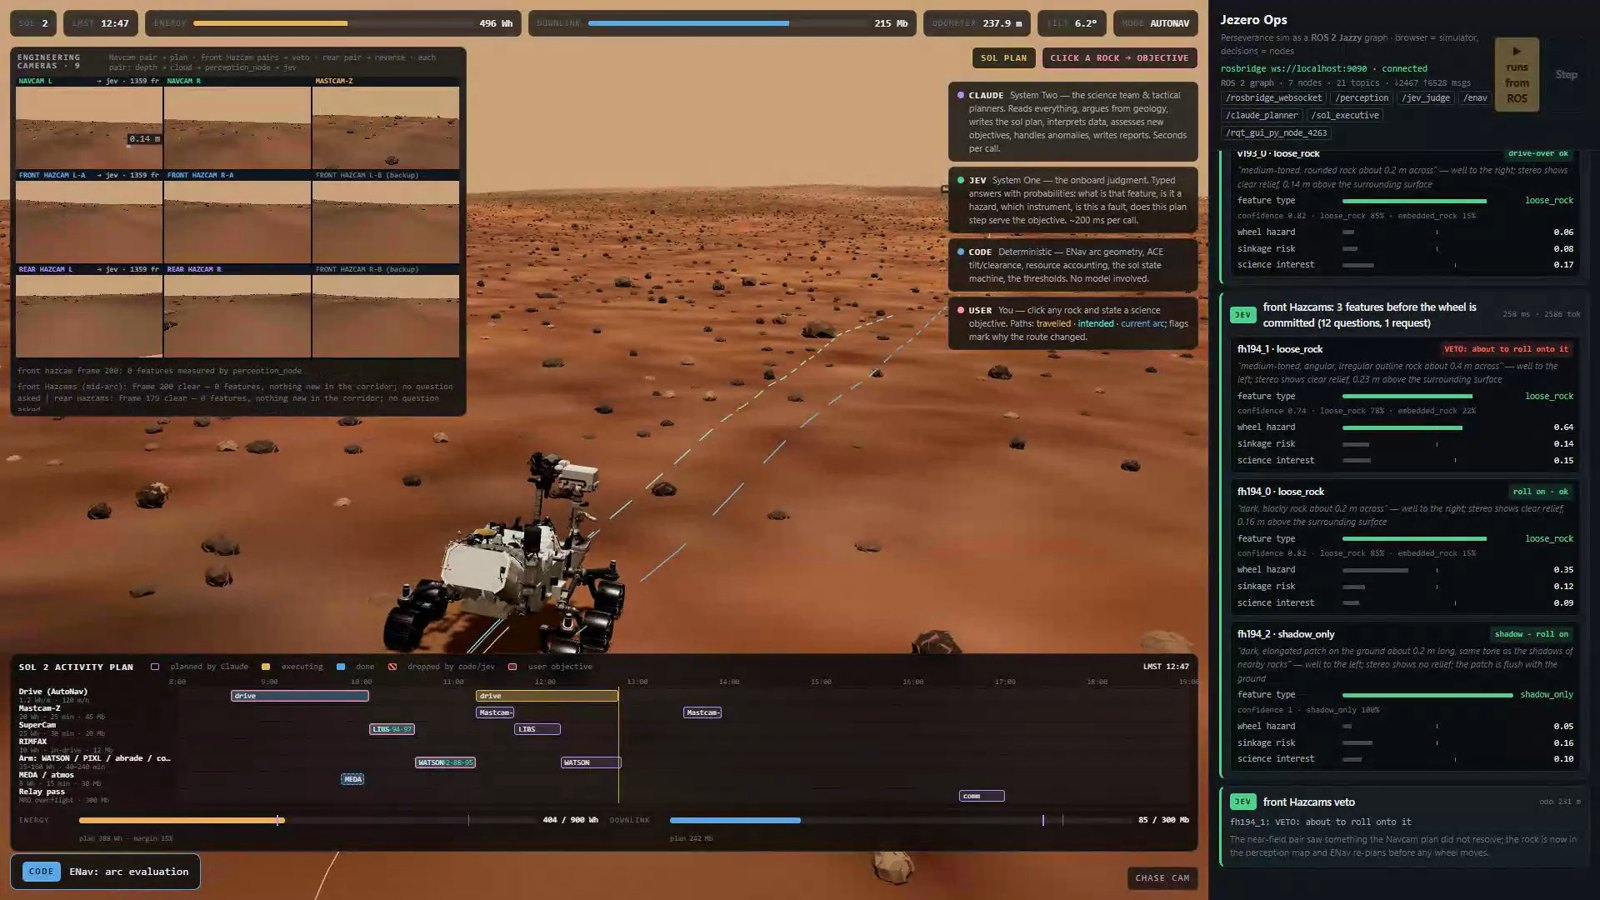
\includegraphics[width=\textwidth]{figs/route-paths.jpg}
\caption{The drive toward Rochette, sol 2, 238\,m on the odometer (ROS\,2 run). The intended route (dashed cyan) and the current arc (blue) run ahead of the rover; the front Hazcam status line in the rig reads ``frame 200 clear --- 0 features, nothing new in the corridor; no question asked''. On the right, a front-Hazcam card from a moment earlier: three features before the wheel is committed, one vetoed at $P(\text{roll-over})=0.64$, one cleared, one a shadow.}
\label{fig:route}
\end{figure}

\subsection{What a flight-like version needs: every camera, before every move}
\label{sec:cameras}
The demo perceives with one mast camera and a depth buffer. Perseverance carries nine engineering cameras: two \textbf{Navcams} on the mast (a stereo pair, about $96^\circ \times 73^\circ$, the planning horizon out to $\sim$20\,m), four \textbf{front Hazcams} (two stereo pairs, one redundant, about $136^\circ \times 102^\circ$, looking down at the ground the front wheels are about to roll onto and the arm workspace), two \textbf{rear Hazcams} (a pair, about $124^\circ \times 102^\circ$, for backing up), and the CacheCam; plus seven science cameras \cite{maki}. Flight AutoNav thinks while driving: it acquires new stereo every few metres, plans the next arc before the current one is finished, and never commands a motion the near-field cameras have not cleared. A flight-like version of this architecture therefore runs jev on \emph{every camera group before every motion command}, and again several times while the arc is executing:

\begin{table}[h]
\centering\small
\begin{tabular}{@{}p{2.6cm}p{2.4cm}p{5.0cm}p{4.6cm}@{}}
\toprule
Camera group & Range / role & jev questions (per feature) & Code gate \\
\midrule
Navcam pair (mast) & 3--20\,m; plan the arc & feature type, wheel hazard, sinkage, science interest & perception map, keep-outs, confidence floor $\to$ re-image \\
\rowrule
Front Hazcam pairs & 0.3--4\,m; ground under and just ahead of the front wheels, arm workspace & \emph{about to roll onto it?} (Noul), \emph{rock or shadow at wheel scale?} (Choice), \emph{arm can deploy?} (Noul) & veto the next step if $P(\text{roll-over hazard})>0.5$; halt if unsure \\
\rowrule
Rear Hazcam pair & 0.3--4\,m behind; reversing & same as front, mirrored & reverse arcs only from what the rear pair has cleared \\
\bottomrule
\end{tabular}
\caption{The three camera groups, what jev is asked about each, and the rule that consumes the answer.}
\end{table}

\begin{figure}[h]
\centering
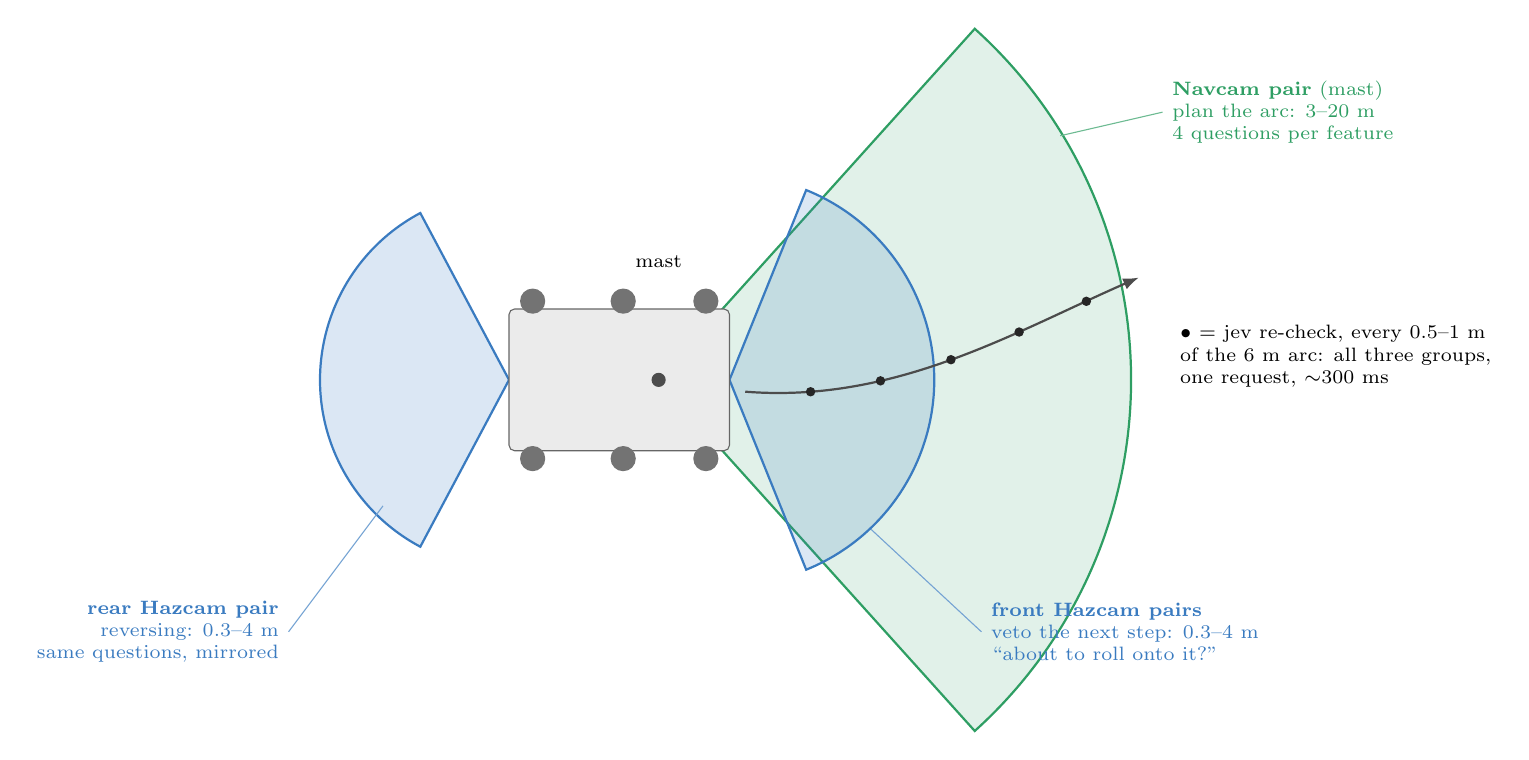
\begin{tikzpicture}[x=1cm, y=1cm, every node/.style={font=\scriptsize}]
% rover body, top view, driving to the right
\fill[black!8, rounded corners=2pt] (-1.4,-0.9) rectangle (1.4,0.9);
\draw[black!60, rounded corners=2pt] (-1.4,-0.9) rectangle (1.4,0.9);
\foreach \x in {-1.1, 0.05, 1.1} { \fill[black!55] (\x,1.0) circle (0.16); \fill[black!55] (\x,-1.0) circle (0.16); }
\fill[black!70] (0.5,0) circle (0.09); \node[font=\scriptsize] at (0.5,1.5) {mast};
% FOV wedges (drawn first so the rover sits on top of them)
\begin{scope}[on background layer]
\fill[jev, opacity=0.14] (0.5,0) -- ++(48:6.0) arc (48:-48:6.0) -- cycle;
\draw[jev, thick] (0.5,0) -- ++(48:6.0) arc (48:-48:6.0) -- cycle;
\fill[code, opacity=0.18] (1.4,0) -- ++(68:2.6) arc (68:-68:2.6) -- cycle;
\draw[code, thick] (1.4,0) -- ++(68:2.6) arc (68:-68:2.6) -- cycle;
\fill[code, opacity=0.18] (-1.4,0) -- ++(118:2.4) arc (118:242:2.4) -- cycle;
\draw[code, thick] (-1.4,0) -- ++(118:2.4) arc (118:242:2.4) -- cycle;
\end{scope}
% labels outside the wedges, with leaders
\node[jev, align=left, anchor=west] (ln) at (6.9,3.4) {\textbf{Navcam pair} (mast)\\plan the arc: 3--20 m\\4 questions per feature};
\draw[jev!70] (ln.west) -- (5.6,3.1);
\node[code, align=left, anchor=west] (lf) at (4.6,-3.2) {\textbf{front Hazcam pairs}\\veto the next step: 0.3--4 m\\``about to roll onto it?''};
\draw[code!70] (lf.west) -- (3.2,-1.9);
\node[code, align=right, anchor=east] (lr) at (-4.2,-3.2) {\textbf{rear Hazcam pair}\\reversing: 0.3--4 m\\same questions, mirrored};
\draw[code!70] (lr.east) -- (-3.0,-1.6);
% the commanded arc and the re-check ticks along it
\draw[black!70, thick, -{Latex[length=2mm]}] (1.6,-0.15) .. controls (3.5,-0.3) and (5.0,0.6) .. (6.6,1.3);
\foreach \t in {0.15,0.32,0.5,0.68,0.86} { \path (1.6,-0.15) .. controls (3.5,-0.3) and (5.0,0.6) .. (6.6,1.3) node[pos=\t, inner sep=0] (p) {}; \fill[black!85] (p) circle (0.06); }
\node[align=left, anchor=west, font=\scriptsize] at (7.0,0.3) {$\bullet$ = jev re-check, every 0.5--1 m\\of the 6 m arc: all three groups,\\one request, $\sim$300 ms};
\end{tikzpicture}
\caption{Camera coverage, top view, and the check cadence. Before any motion command all three groups must have been cleared; during the 6\,m arc the near-field pairs are re-asked every 0.5--1\,m, so a rock that was below the Navcam's stereo threshold at 8\,m is caught by the front Hazcams at 1\,m before a wheel reaches it.}
\label{fig:cameras}
\end{figure}

The point of the cadence is that it is only affordable with a System One. A Hazcam check is a handful of features, three questions each, one request, about 200--300\,ms; that is cheaper than the stereo correlation that feeds it, so the rover can afford to ask before every step and several times per arc --- the same ``look, then move, then look again'' discipline rover operations already use, with the looking done by a calibrated judge instead of a threshold on a height map. An LLM in that seat would be a hundred times too slow and would not return a number a veto rule could read. In the ROS\,2 port (Section~\ref{sec:ros2}) this becomes three perception nodes feeding one judge service, with the executive's motion command gated on all three having answered since the last odometry tick.


\begin{figure}[p]
\centering
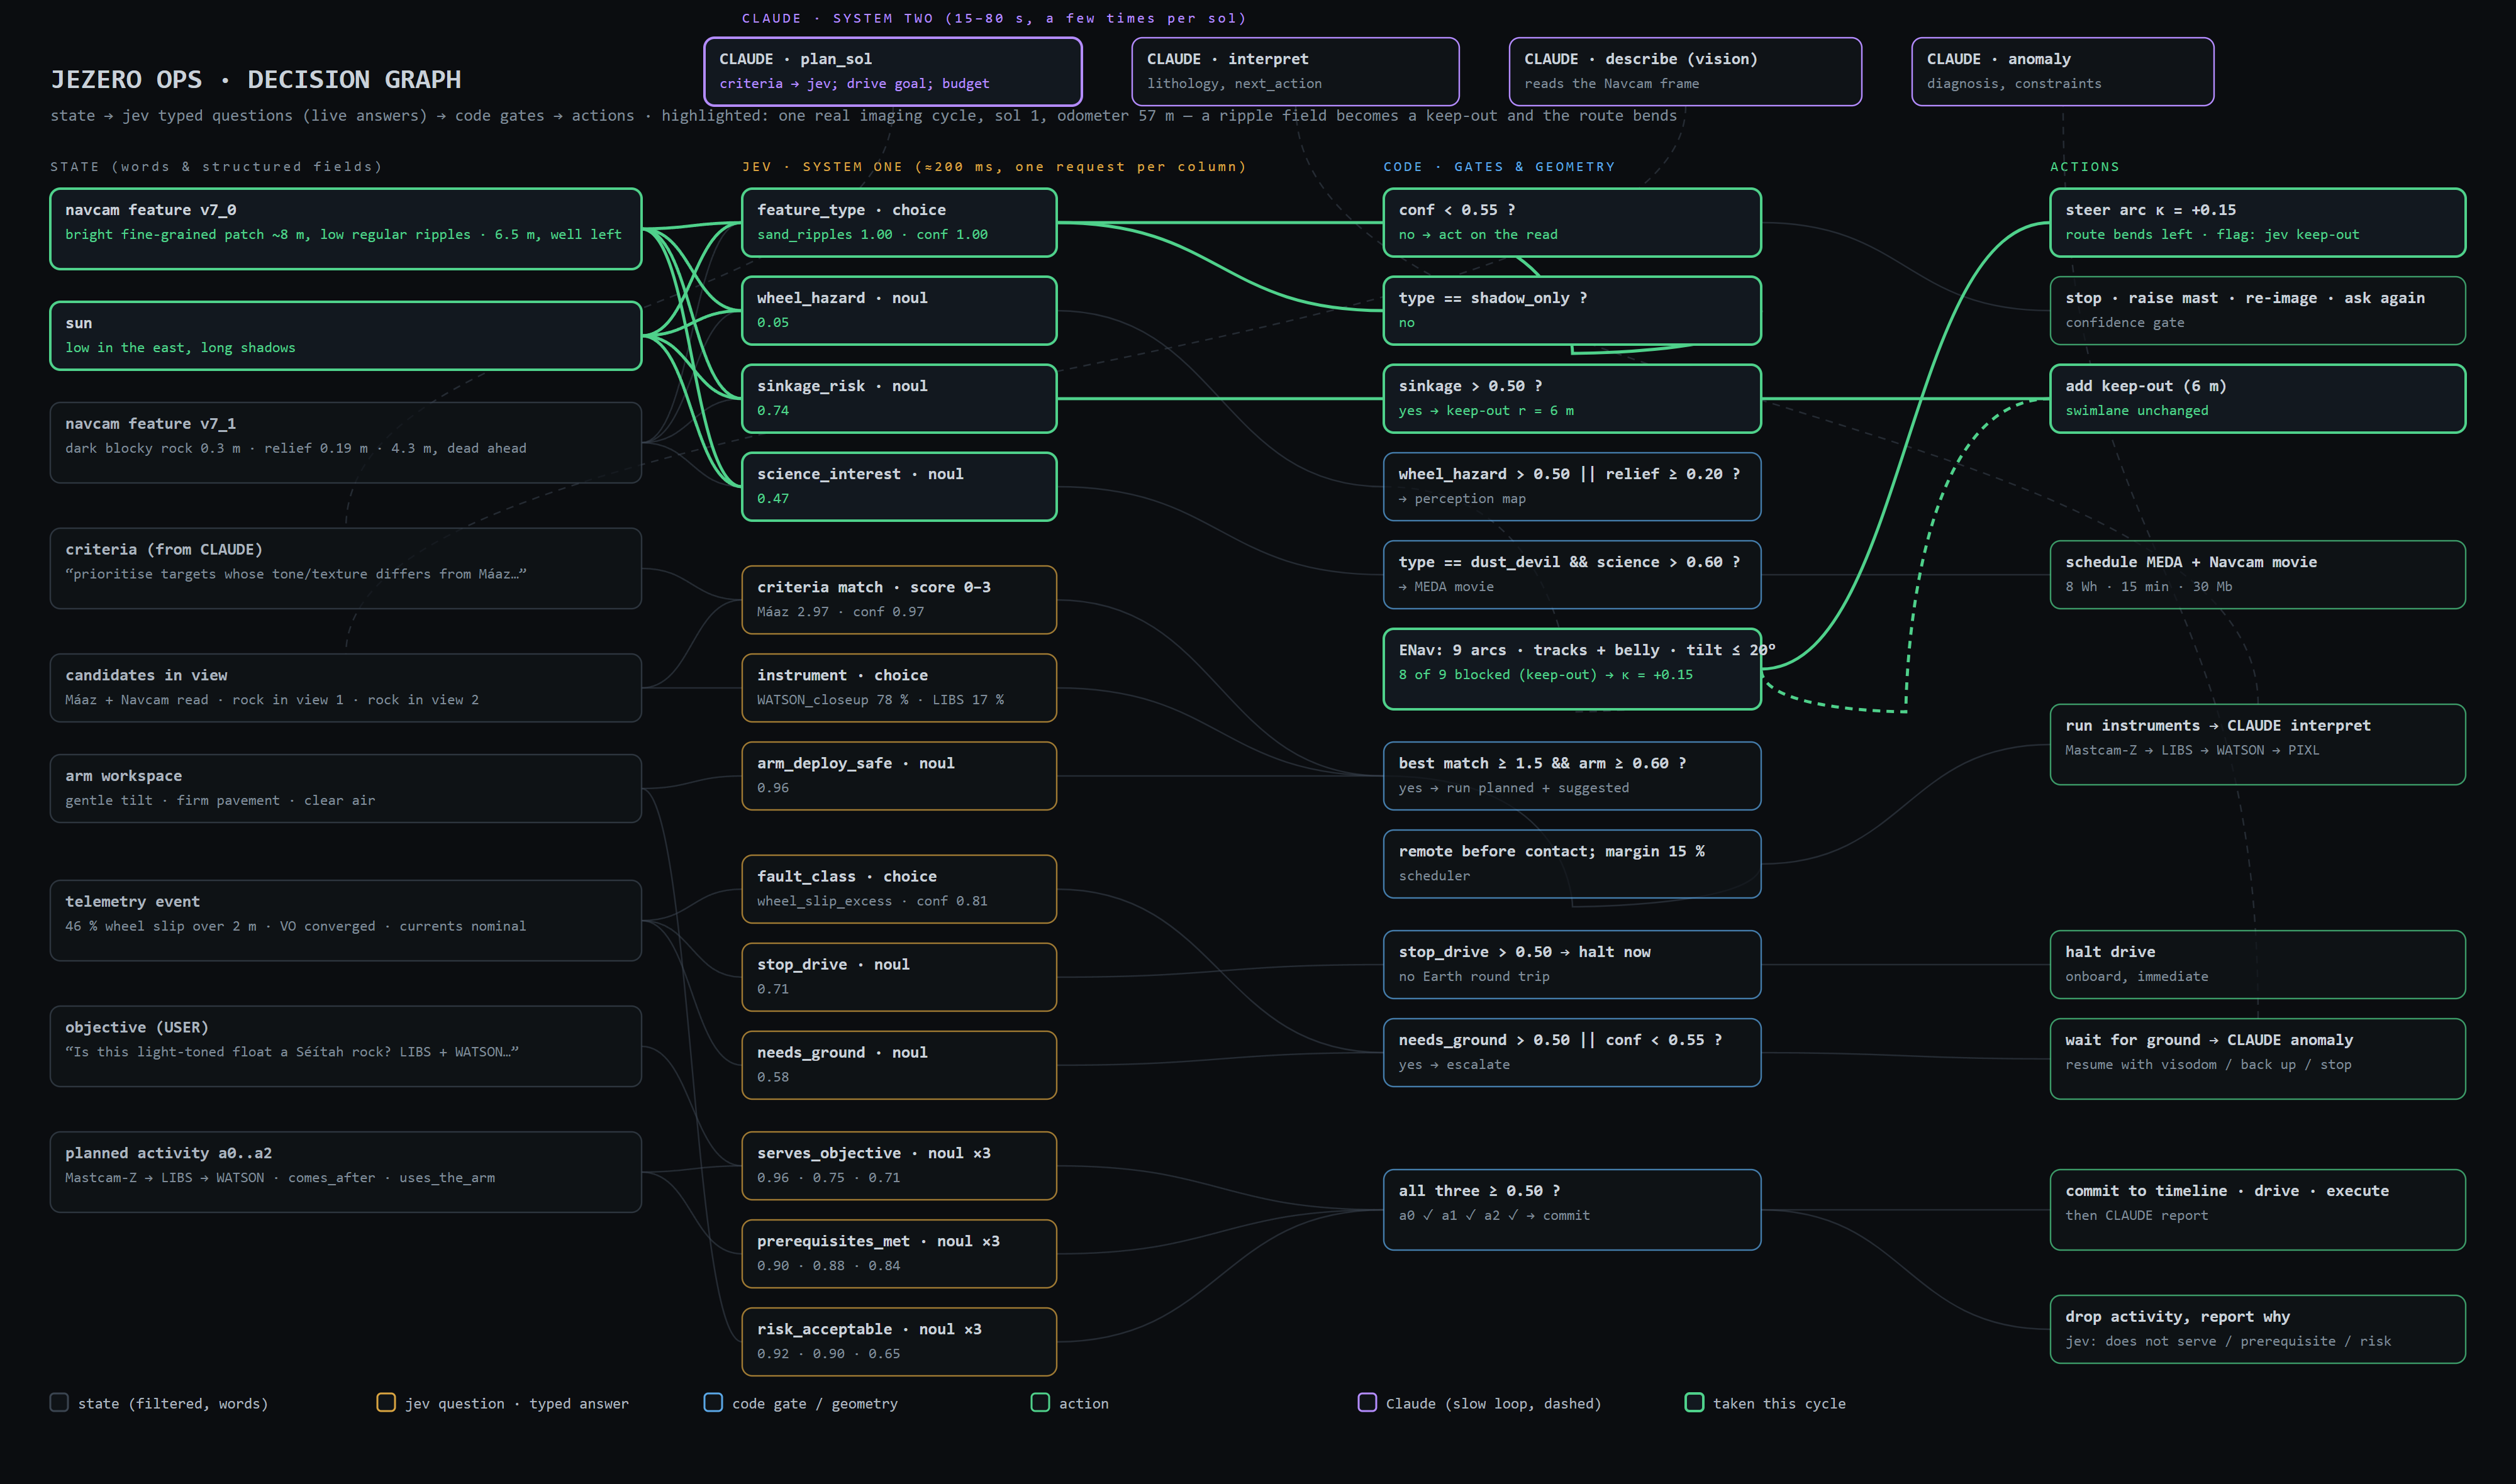
\includegraphics[width=\textwidth]{decision-graph.png}
\caption{The rover's decision graph in the style of TypeSafe's own demos. Left: the filtered state jev is shown (words, not raw numbers). Middle: jev's typed questions with their live answers --- a Choice returns an option and a confidence, a Noul a probability, a Score a position on ordered levels. Then the code gates that turn those numbers into actions, and the actions themselves. Claude's slow loop runs across the top and touches the graph only at its edges: it writes the criteria the middle column applies, and it reads the results. The lit path is a real cycle from the recorded run: a bright ripple field $\rightarrow$ \texttt{sand\_ripples} 1.00 / \texttt{sinkage\_risk} 0.74 $\rightarrow$ keep-out 6\,m $\rightarrow$ ENav finds 8 of 9 arcs blocked and steers $\kappa=+0.15$.}
\label{fig:graph}
\end{figure}

\subsection{Science stops: vision belongs to the LLM}
At a target the Navcam frame goes to Claude, which reads the image and returns a field-geologist's description --- tone, texture, coating, size relative to a wheel, other rocks in frame, hazards noticed --- appended to the target's state. Then jev does what AEGIS does on the real rover: it scores each visible candidate against the team's criteria (a four-level Score), picks the instrument (a Choice), and judges whether arm deployment is safe now. Code enforces the ordering and the scheduler margin, runs the instruments, and hands the results to Claude, which interprets them against the hypotheses and may amend the plan (M\'aaz: basalt, supports H1, float --- not a coring candidate; abrade for texture, hold the tube for Rochette). Figure~\ref{fig:rochette} shows the same loop at Rochette in the ROS\,2 run.

\begin{figure}[p]
\centering
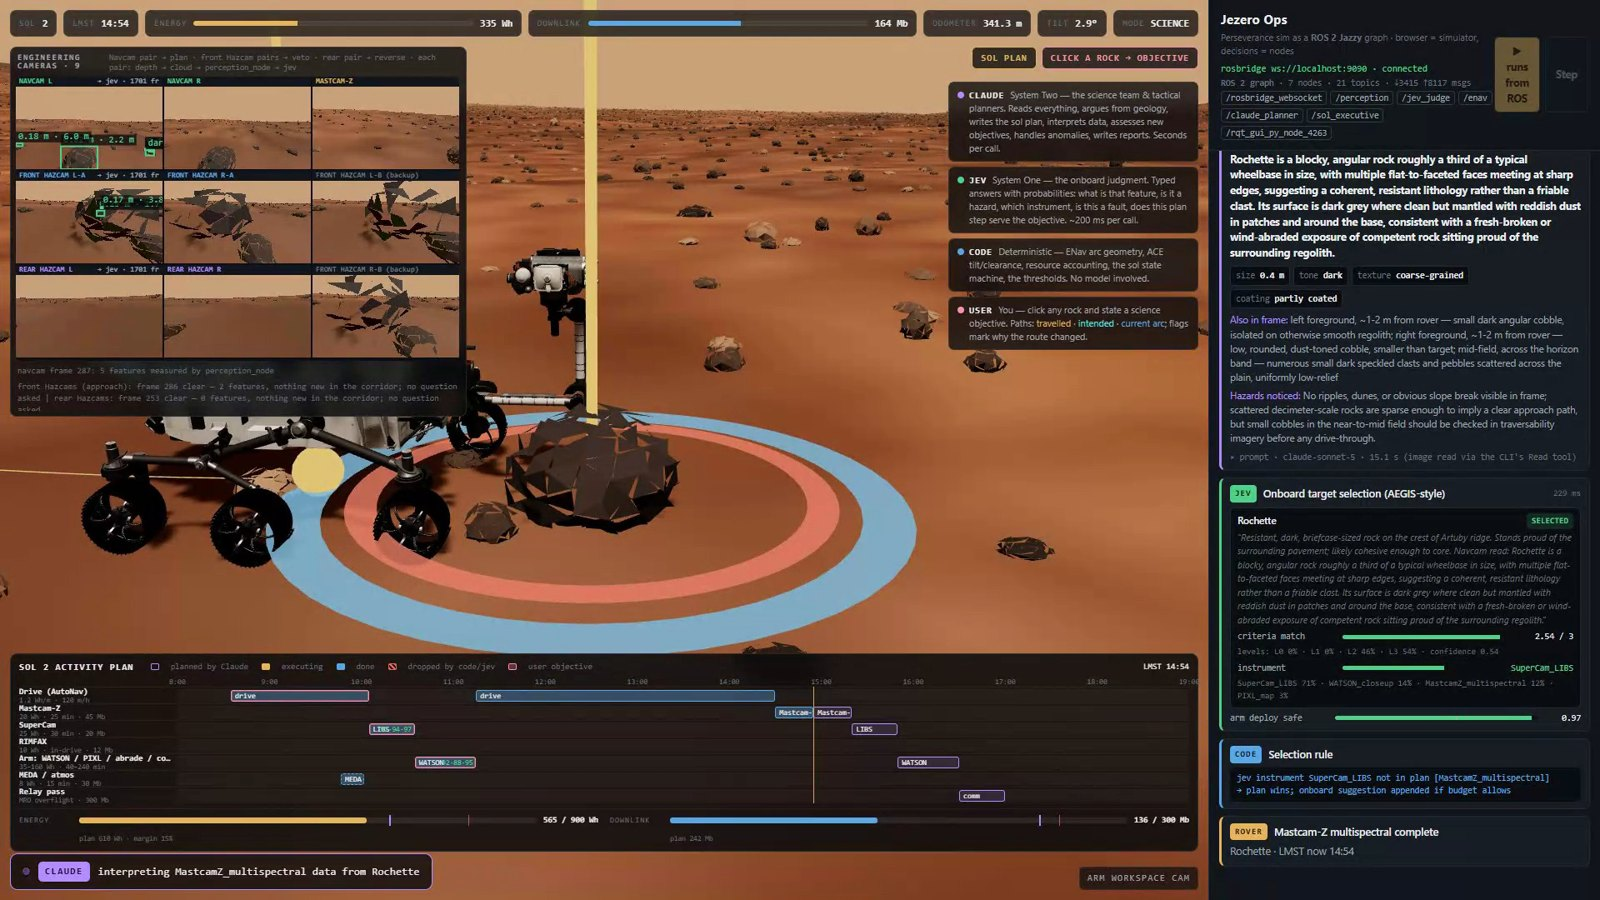
\includegraphics[width=\textwidth]{figs/rochette-science.jpg}
\caption{The science stop at Rochette, sol 2 (ROS\,2 run). Claude has read the Navcam frame through the \texttt{/claude/describe} service --- \emph{blocky, angular rock roughly a third of a wheelbase in size \ldots coherent, resistant lithology}, coarse-grained, partly coated, hazards noticed: none --- and that description is appended to the target's state. jev then scores it against the team's criteria (2.54/3, confidence 0.54), picks SuperCam LIBS (71\,\%) and clears the arm (0.97); code applies the selection rule (the plan wins, the onboard suggestion is appended if budget allows). The rig shows both Hazcam pairs measuring the cobbles around the target.}
\label{fig:rochette}
\end{figure}

\subsection{Objectives from a human, verified before they cost anything}
Click any rock and type what should be checked. Claude assesses (worth it? which instruments? what does it displace? inside the remaining Wh/Mb/minutes with margin); jev verifies \emph{every planned activity} with three probabilities --- serves the objective, prerequisites met, risk acceptable now, floor 0.5; code commits the survivors to the swimlane, drives, executes; Claude files a report: confirmed / refuted / inconclusive, evidence, cost, recommendation. In one take, on a light-toned float rock, LIBS and WATSON returned olivine and carbonate and the report read \emph{S\'e\'itah-derived, confirmed (high)}. In another, on a dark float: \emph{refuted --- ordinary basalt; WATSON correctly withheld; Rochette budget untouched}. Figures~\ref{fig:objective} and \ref{fig:objtarget} show the moment of injection and the assessment.

\begin{figure}[p]
\centering
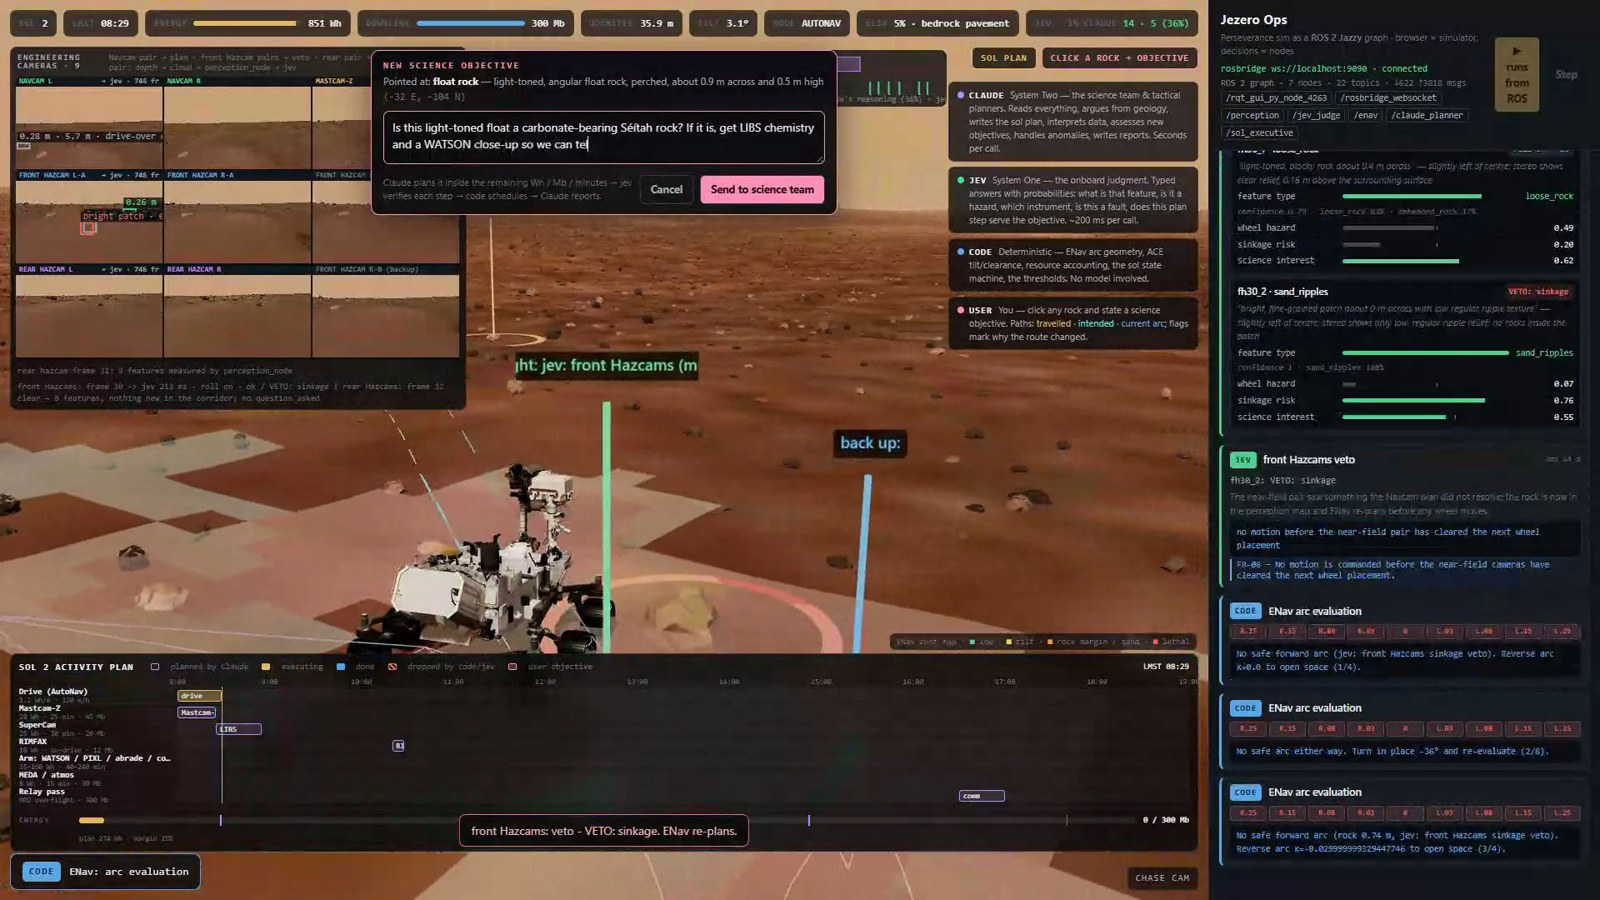
\includegraphics[width=\textwidth]{figs/objective-entry.jpg}
\caption{Injecting an objective mid-drive, sol 2 (ROS\,2 run). The user has clicked a light-toned float rock 16\,m ahead (its description and position are filled in from the pick) and is typing the question, which the browser publishes on \texttt{/ops/user\_objective}. Behind the panel the rover is mid-manoeuvre: a front-Hazcam sinkage veto (\texttt{sand\_ripples} 1.00, $P(\text{sinkage})=0.76$, FR-06) has just made ENav reverse and turn in place; the cost map and the Hazcam frusta are visible under the dialog.}
\label{fig:objective}
\end{figure}

\begin{figure}[p]
\centering
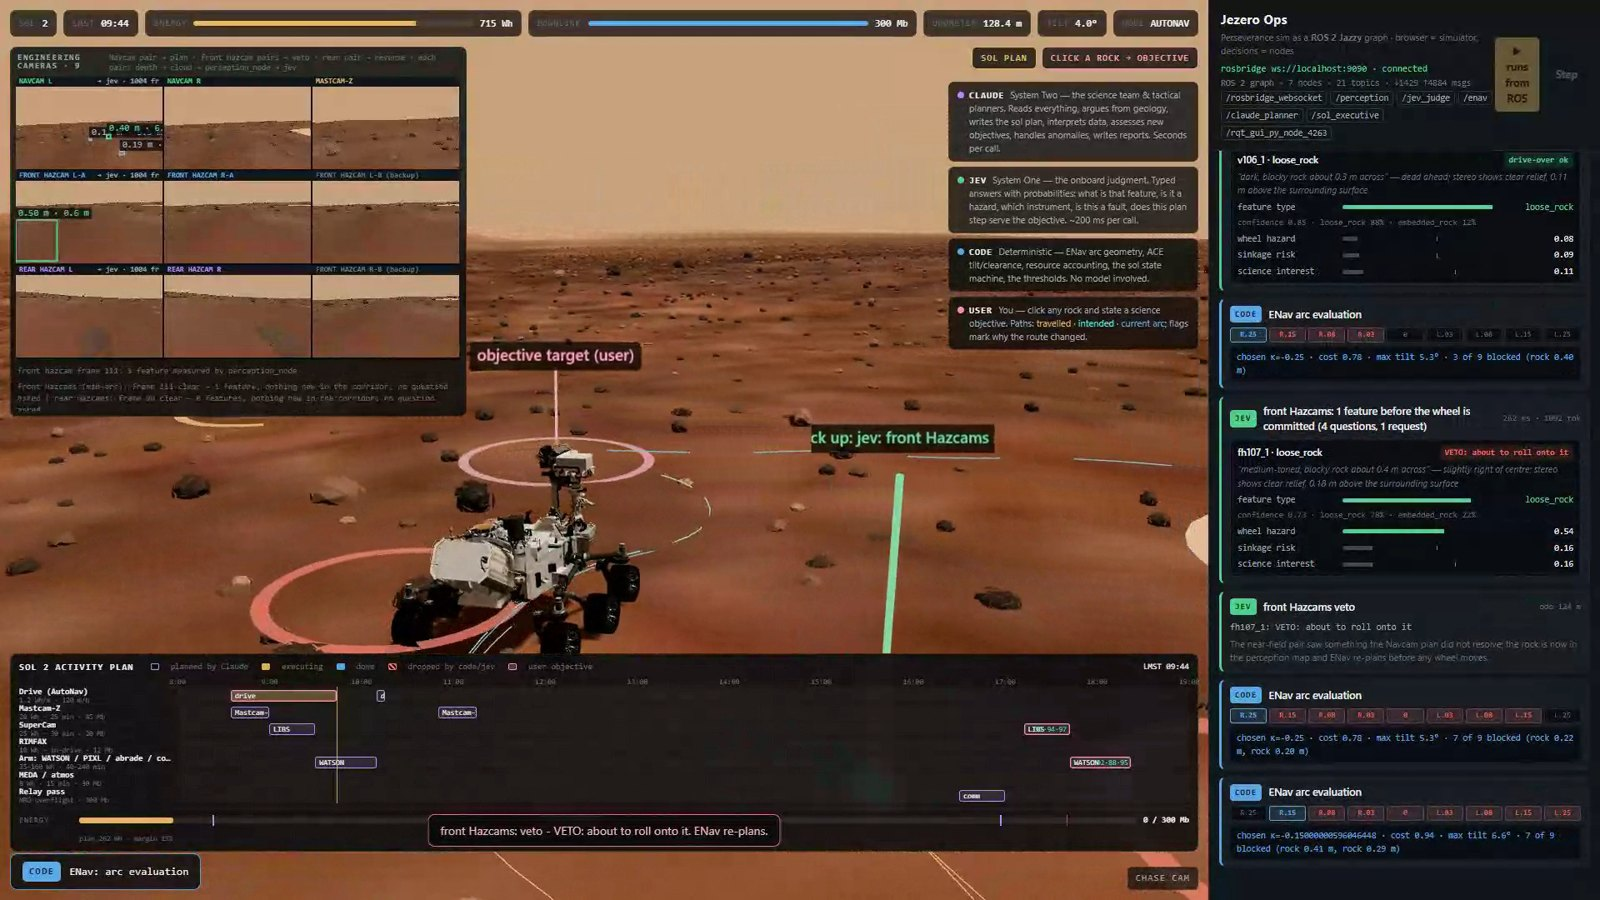
\includegraphics[width=\textwidth]{figs/objective-target.jpg}
\caption{The objective in the system (ROS\,2 run): the picked rock flagged \emph{objective target (user)} ahead of the rover, the approach drive under way, a front-Hazcam veto flag (``back up: jev: front Hazcams'') planted on the track where a 0.4\,m rock at $P=0.54$ stopped a segment, and the swimlane carrying the objective's LIBS and WATSON blocks with jev's three verification probabilities.}
\label{fig:objtarget}
\end{figure}

\subsection{Faults: onboard halts, Earth decides}
A scripted 46\,\% wheel-slip event is triaged by jev in one request: \texttt{fault\_class} (Choice), \texttt{stop\_drive} (Noul), \texttt{needs\_ground} (Noul). Code halts immediately if $P(\text{stop})>0.5$ --- no Earth round trip for a halt --- and escalates to Claude only if $P(\text{needs ground})>0.5$ or the classification is under the confidence floor. Claude diagnoses and returns constraints the planners can encode.


\section{System One inside System Two}
\label{sec:inside}
The first two builds kept the two speeds apart: Claude planned at the cadence of a sol, jev judged at the cadence of a wheel, and code passed messages between them. That is the flight-operations picture, and it is right. But it hides a question the demonstration is meant to answer: \emph{how much of the slow mind's reasoning can, and should, be fast judgment?} Ground planners do not reason in a vacuum; they lean on onboard tools --- AEGIS scores, slip tables, keep-out maps --- and the cheapest way to check a draft plan is to ask the same judge the rover will use.

So in this version jev is also a tool \emph{inside} Claude's reasoning. The Claude CLI is launched with an MCP server (\texttt{tools/mcp\_jev\_server.mjs}) that exposes one tool, \texttt{ask\_jev(state, questions)}: the same TypeSafe call the rover makes, returned to the model as evidence mid-thought. The prompts tell Claude what a planner would do with such a tool --- score every candidate target against the draft criteria before committing them, check an activity order against the sequencing rules, break a tie between two next actions, check whether an activity actually bears on a human's objective --- and to treat the answers as evidence to weigh, not commands. Every consultation is captured from the CLI's event stream and returned to the executive (\texttt{consults\_json}), so the console shows it under the Claude card it belongs to, the HUD counts it, and the ``two speeds of mind'' strip draws it as a green tick inside the purple thinking block (Figures~\ref{fig:mind} and \ref{fig:graph2}).

\begin{figure}[p]
\centering
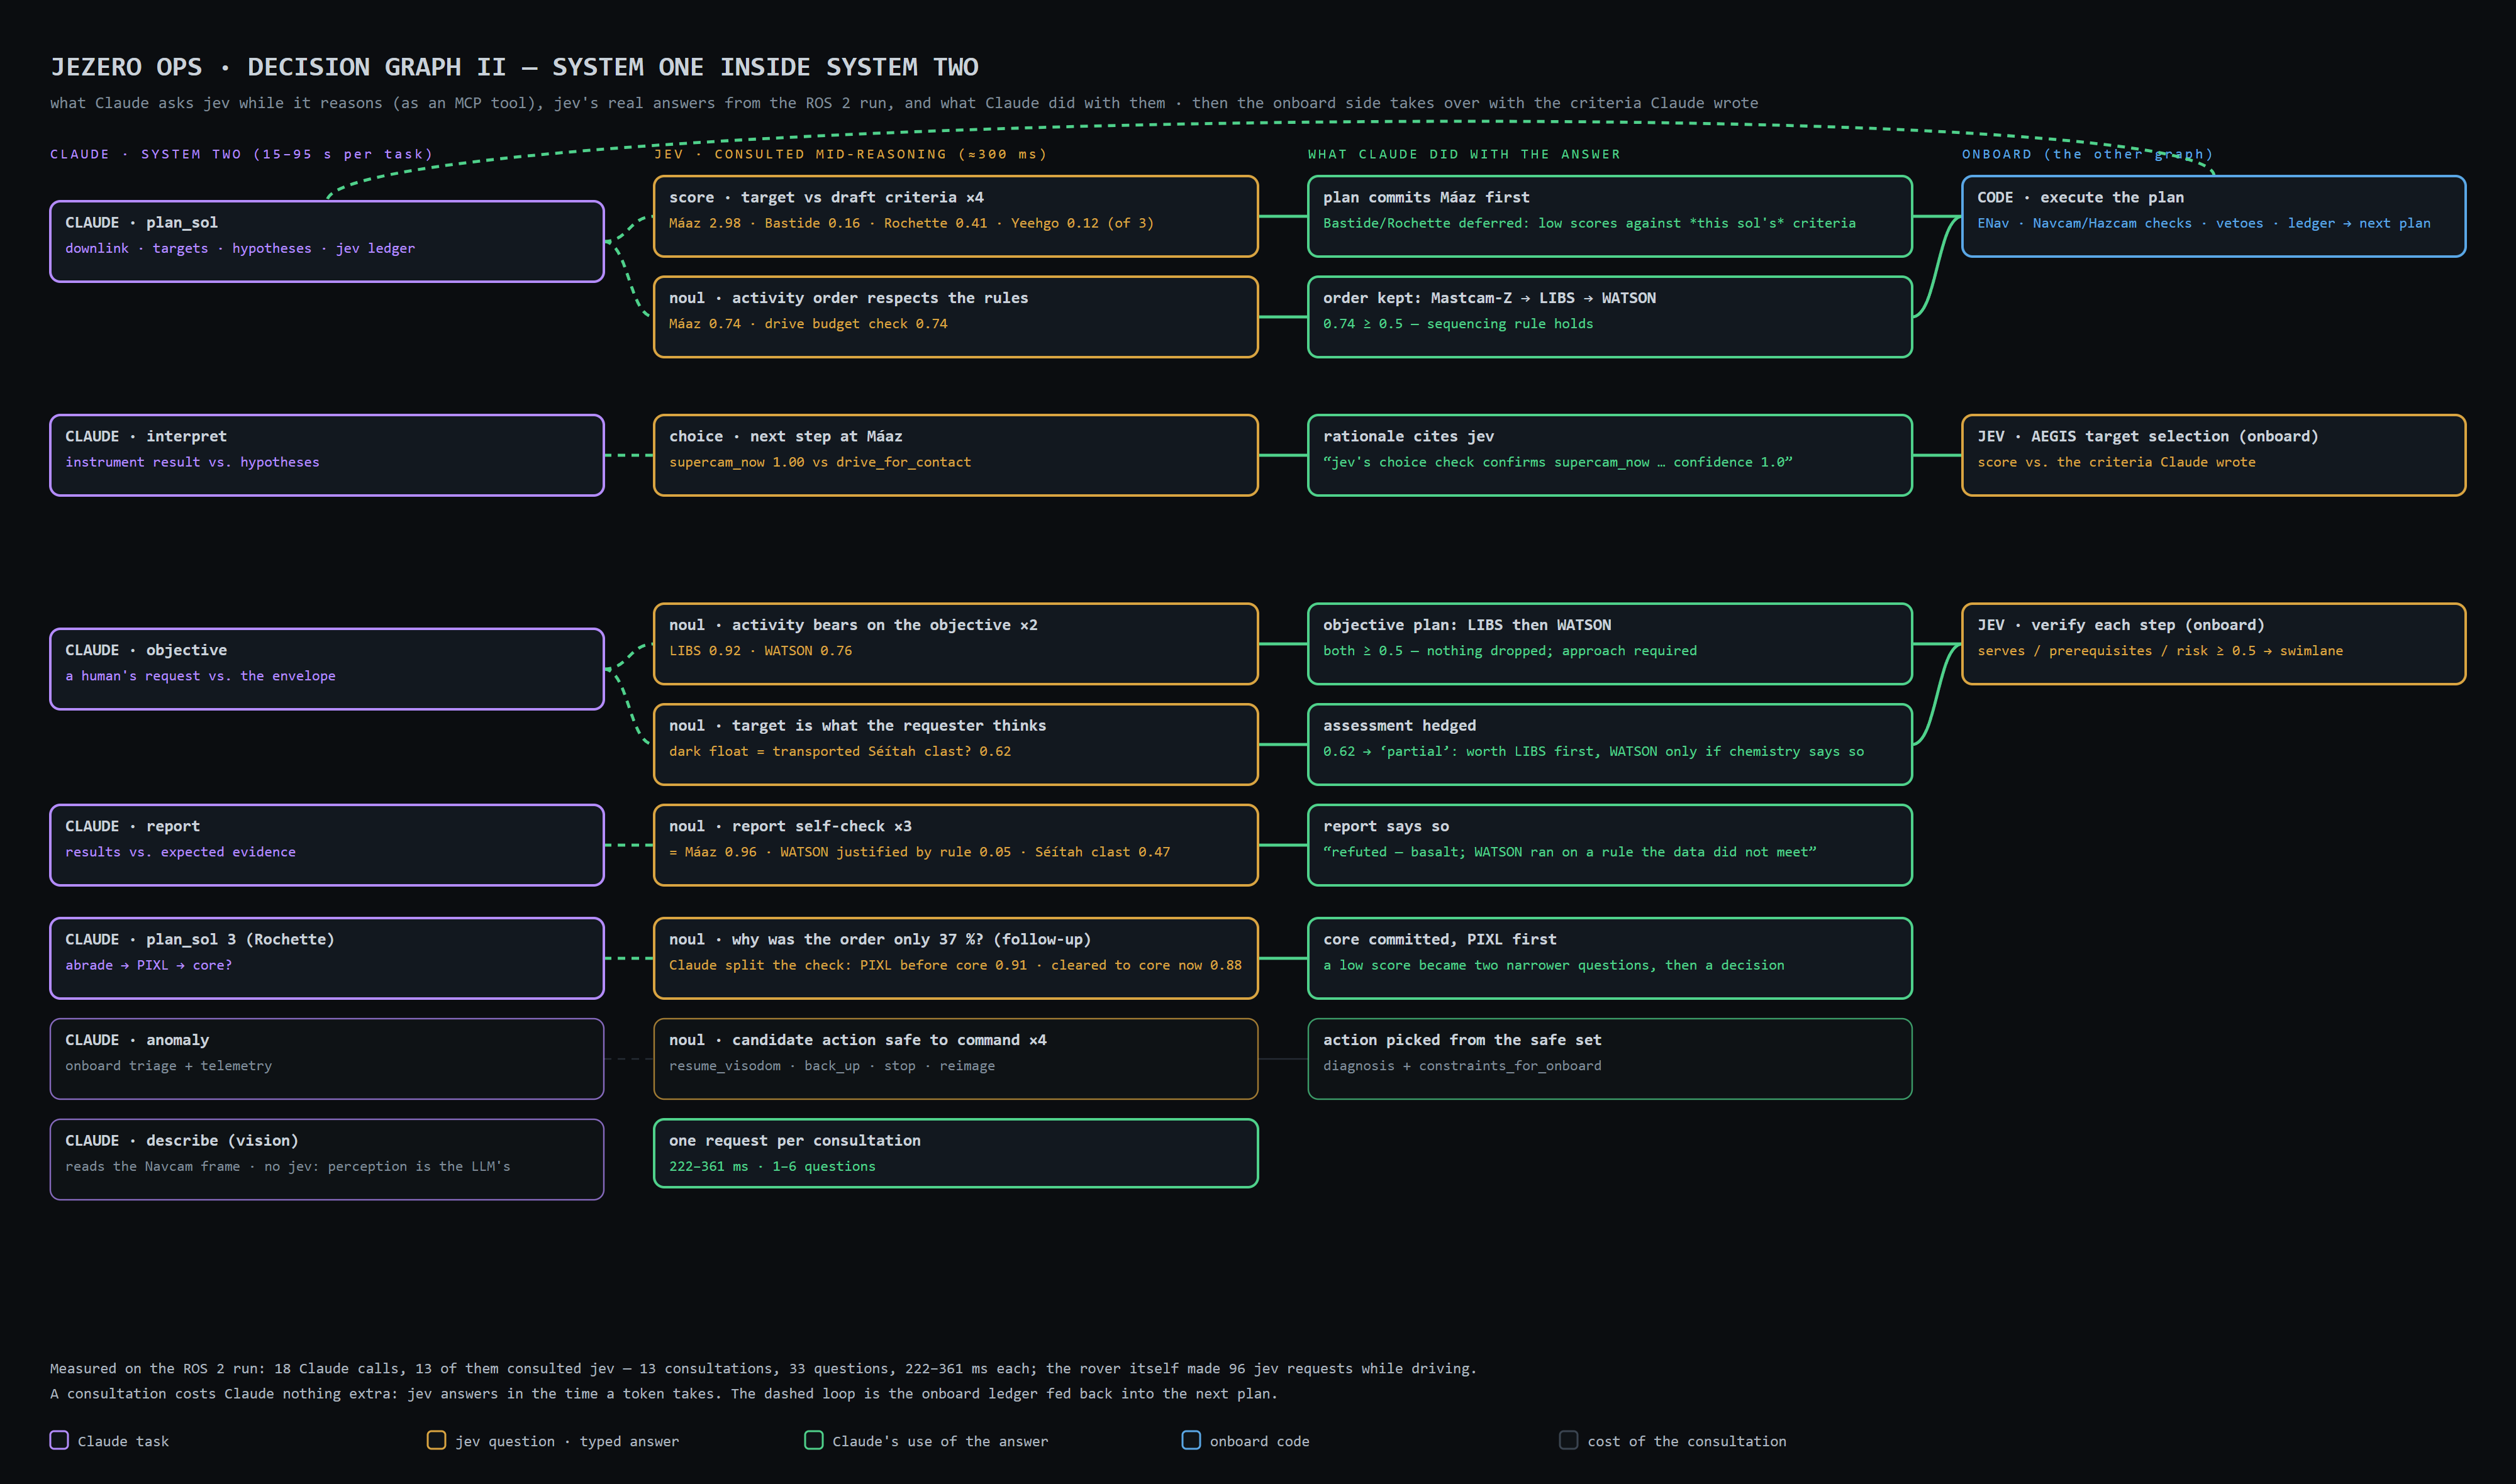
\includegraphics[width=\textwidth]{decision-graph-2.png}
\caption{Decision graph II: what Claude asked jev while it reasoned, jev's real answers from the ROS\,2 run, and what Claude did with them. Planning sol 1 it scored all four targets against its own draft criteria (M\'aaz 2.98 of 3, Bastide 0.16) and checked its ordering (0.74); interpreting M\'aaz it asked one Choice to break a tie and cited the answer in its rationale; assessing the user's objective it asked whether each activity bears on it (LIBS 0.92, WATSON 0.76) and whether the rock is what the requester thinks (0.62 --- so it hedged); writing the report it asked jev to check its own conclusion and got told WATSON had not been justified by its own rule (0.05) --- and said so. Planning sol 3 it got a low ordering score, asked \emph{why} with two narrower questions, and committed the core with PIXL first.}
\label{fig:graph2}
\end{figure}

\subsection{How much is real time?}
Measured on the recorded run: \textbf{13 Claude calls (9 planning and interpretation, 4 vision reads), and every one of the 9 that was told it could consult jev did so --- 9 consultations, 39 typed questions, 252--345\,ms each}. Against that, the rover itself made 760 jev calls carrying about 2\,900 typed questions. So the in-Claude share is now about 1\,\% of all System One calls, and it is worth being exact about why that fell from the 12\,\% an earlier pass measured: not because the planner consults less, but because the onboard cadence rose roughly eightfold once the whole camera rig and the whole telemetry stream started going to jev. A consultation still adds under half a second to a call that takes 15--125\,s: jev answers in the time a token takes. The other direction is the ledger: at every uplink Claude is told what jev decided while driving --- frames judged, obstacles and keep-outs added, vetoes, reads below the confidence floor, the ground classes seen --- so the slow mind plans on what the fast mind found.

\subsection{What the demo shows about the split}
Three things the consultations did that neither engine could do alone. \emph{Calibrated doubt on Claude's own draft}: jev scored Rochette 0.41 against sol-1 criteria written for M\'aaz, and the plan deferred it --- a planner's draft was checked by the onboard judge before uplink. \emph{An honest audit of Claude's report}: asked whether its WATSON run was justified by the rule it had itself set (``only if the chemistry says so''), jev said 0.05, and the report says the run was not warranted. \emph{Decomposition under uncertainty}: a low ordering score became two narrower questions (PIXL before core? cleared to core now?) rather than a guess. None of this is jev reasoning --- it cannot --- and none of it is Claude judging its own calibration --- it cannot. The reasoning stays in System Two; the calibrated judgment stays in System One; the boundary now runs \emph{through} the LLM's chain of thought, and it is still drawn in code and visible on screen.

\section{What the port borrowed from JPL}
\label{sec:jpl}
The second pass added the parts of real rover practice the first build only gestured at.
\begin{itemize}
\item \textbf{Flight rules, cited.} Every gate the code applies now names the rule it enforces (FR-01\ldots FR-14: ops window, 15\,\% margin, tilt limit, step limit, keep-outs, near-field clearance before motion, reverse only on imaged ground, the confidence floor, arm deploy conditions, sequencing, onboard halt vs.\ ground escalation, objective verification, the planned final bump, slip-budgeted driving). Modelled on the way MER, MSL and M2020 planners work under enumerated flight rules; the numbers are this simulation's.
\item \textbf{Slip prediction by terrain class.} jev is asked one more question per Navcam frame --- what kind of ground the wheels will roll on: bedrock pavement, cobble field, mixed regolith, sand drift --- and code maps the class to a predicted slip (5 / 12 / 20 / 45\,\%) that inflates the energy and time each metre costs, the way MSL and M2020 planners size a drive from slip-vs-terrain tables. The HUD shows it.
\item \textbf{A traversability cost map.} ENav publishes the hazard map it plans on (tilt fraction, rocks in the perception map with a margin, keep-outs, sand; 0--100) and the simulator draws it over the terrain, so the console shows \emph{why} arcs are blocked, not only that they are --- the ACE/ENav picture rather than a black box.
\item \textbf{The nine-camera cadence} (Section~\ref{sec:cameras}), with each pair's field of view drawn for a moment when it is asked to image.
\item \textbf{The onboard ledger} in the next uplink, so the sol plan is written from what the rover actually judged.
\end{itemize}

\begin{figure}[p]
\centering
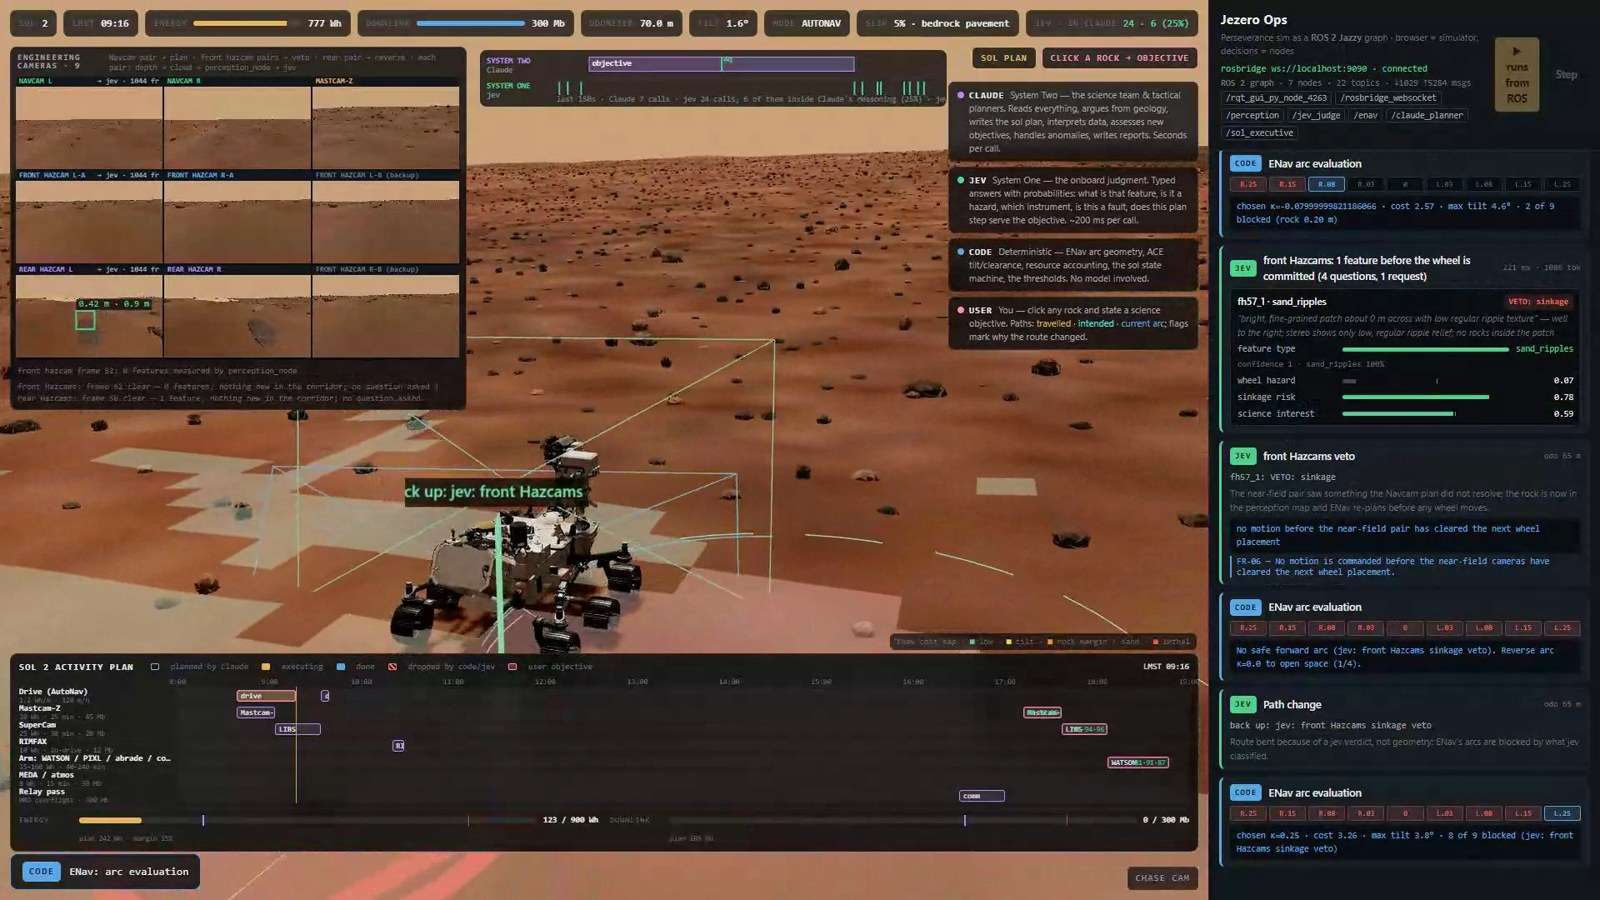
\includegraphics[width=\textwidth]{figs/costmap-veto.jpg}
\caption{ENav's cost map and a Hazcam veto, sol 2 (ROS\,2 run). The translucent cells around the rover are the traversability map ENav plans on --- green low, yellow tilt, orange rock margin or sand, red lethal (legend bottom right); the blue lines are the fields of view of the camera pairs just asked to image. The front Hazcam pair has found a bright ripple patch under the next wheel placement; jev answered \texttt{sand\_ripples} at confidence 1.00 with $P(\text{sinkage})=0.79$, the executive vetoed the segment citing FR-06, ENav found eight of nine arcs blocked and chose a reverse arc. The HUD reads predicted slip 5\,\% on bedrock pavement and 24 jev calls so far, 6 of them inside Claude's reasoning; the strip shows the objective assessment in progress. The flag on the track reads \emph{back up: jev: front Hazcams}.}
\label{fig:costmap}
\end{figure}

\begin{figure}[p]
\centering
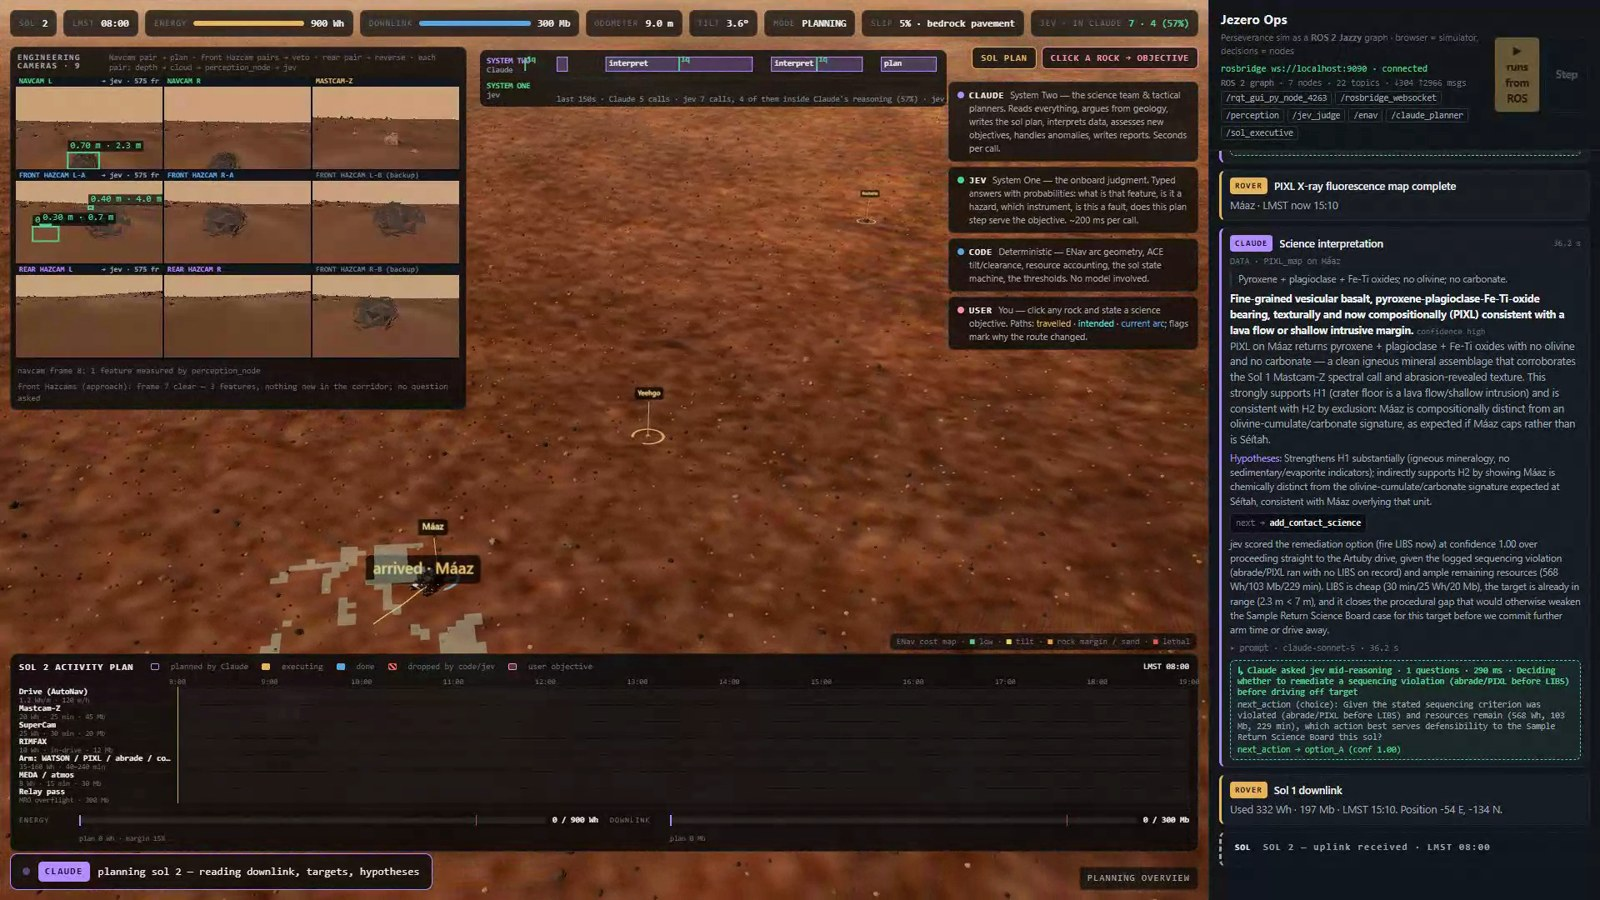
\includegraphics[width=\textwidth]{figs/mind-strip.jpg}
\caption{The ROS\,2 page during sol-2 planning. Top centre: the ``two speeds of mind'' strip --- Claude's thinking intervals as purple blocks (\emph{describe}, \emph{interpret}, \emph{plan}), jev's onboard calls as green ticks on the lower lane, and the consultations Claude made \emph{inside} its reasoning as green ticks inside the purple blocks. Top right of the HUD: predicted slip for the ground ahead and the jev counters (calls · inside Claude). Right: Claude's PIXL interpretation card with the consultation it made rendered beneath it --- having noticed that abrade and PIXL had run without a LIBS reading (a sequencing violation on its own record), it asked jev one Choice, \emph{remediate now or drive off?}, got \texttt{option\_A} at 1.00, and its rationale says so. HUD: 7 jev calls so far, 4 of them inside Claude (57\,\%). Top left: the ENav cost map over the terrain.}
\label{fig:mind}
\end{figure}


\section{Flight-like: actions, a behaviour tree, and jev on every stream}
\label{sec:flight}
The last pass made the graph the shape a rover team would recognise, and used jev everywhere a real rover would use a fast calibrated judge.

\paragraph{Topics, services, actions.} Sensors and state are topics (\texttt{/rover/state} 10\,Hz, \texttt{/rover/telemetry} 1\,Hz, the camera clouds, the cost map, the console streams). Every jev judgment is a \emph{service}: 200--500\,ms, no intermediate state, never worth cancelling. Every Claude call is an \emph{action}: 15--105\,s, observable progress (phase, turns, jev consultations, elapsed --- streamed to the ``two speeds'' strip), and cancellable --- the executive holds the goal handle and withdraws it when the situation changes; the server kills the CLI and the question is re-asked against the current state. The rule is the flight-software one: a judgment is a service, a behaviour is an action.

\paragraph{The executive is a behaviour tree.} \texttt{py\_trees}: a no-memory Selector whose first child is the safety condition and whose second is the mission Sequence --- PlanSol, ReviewPlan, ExecuteSol, Downlink --- each a leaf that runs in a thread and reports RUNNING. The tree ticks at 2\,Hz, publishes its state to \texttt{/ops/tree} and is drawn on the page (Figure~\ref{fig:flight}). The safety branch \emph{reports} a halt rather than preempting the mission: the halt and the anomaly action are handled inside the executing leaf, and a real preempt (our first version) cancelled the very action handling it and reset the sequence. The immediate halt does not wait for a tick either: stop verdicts are latched and the drive loop consumes them before every segment --- the scripted slip lasts seven seconds, and an unlatched check missed it once.

\paragraph{jev on the telemetry stream.} A \texttt{health\_monitor} node turns the housekeeping stream --- state of charge, battery temperature, the highest actuator current, wheel slip, visual-odometry status, tilt, suspension differential, dust opacity --- into words at 1\,Hz and asks jev three questions whenever the words change or every 10\,s while driving: what does this indicate (eight classes), should the drive stop, does the ground need to decide. $P(\text{stop})>0.5$ halts the next segment (FR-11); $P(\text{ground})>0.5$ starts the Claude anomaly action; a change of fault class while that action is running cancels it and re-issues it. The scripted slip event now arrives the way it would on a rover: as telemetry.

\paragraph{jev everywhere else.} Before uplink, jev reviews every planned activity of the sol the way a sequence review board would (serves the intent, in order, acceptable risk); what fails is dropped and reported. Every Navcam frame is judged usable or not before the rover plans on it. Before any core, jev is asked whether the sample would be defensible to the Sample Return Science Board on the evidence in hand, whether the rock will yield an intact core, and what is missing if not. At every relay pass, jev scores each data product's value to the hypotheses if it comes down now, and code fills the pass by score, minus an engineering reserve. Figure~\ref{fig:graph3} lists all fourteen uses with their cadence and the rule that consumes each answer; none of them asks jev what to do next.


\paragraph{The arm, placed by code, judged by jev.} Contact science used to be a two-joint gesture and a timer. The NASA model's arm is a real chain --- shoulder azimuth and elevation, elbow, wrist, turret --- and the simulator now drives it with a cyclic-coordinate-descent inverse-kinematics solver with joint limits, so the turret actually travels to the rendered rock (Figure~\ref{fig:arm}). The placement decision is split the way the rest of the system is split. Code derives candidate spots from the rock's geometry --- top facet, the face turned toward the rover, the two flanks --- and describes each in words: attitude, reach against the workspace, light from the sun's position, dust, roughness, height. jev scores every spot for the instrument (a Score on four levels) and flags collision risk (a Noul), one request. Code takes the best acceptable spot, unstows, and brings the turret to a hover thirty centimetres over it, along the surface normal. From there the workspace is read back in words --- the placement-solution error, the surface tilt under the instrument, the clearance --- and jev is asked whether it is safe to lower to contact and whether the data will be good. Only then does the turret touch the rock; a no-go tries the next spot once, then stows. In the recorded run jev cleared the placements it was asked about (safe-to-contact 0.57 and 0.59 on the tilted tops of M'aaz and the user's rock, answering ``shift'' each time; there was no other acceptable spot, so code proceeded and said so) and scored Rochette's flat top 2.99 of 3. In an earlier take it refused a steeply tilted top outright --- safe-to-contact 0.26 --- and the arm stowed with the reason on the console. Two more closed questions, two more rules citing FR-09, and the arm never moves on a judgment alone: the spot came from geometry, the motion from kinematics, and jev said yes or no at the two places a flight team would want a fast, calibrated opinion.

\begin{figure}[p]
\centering
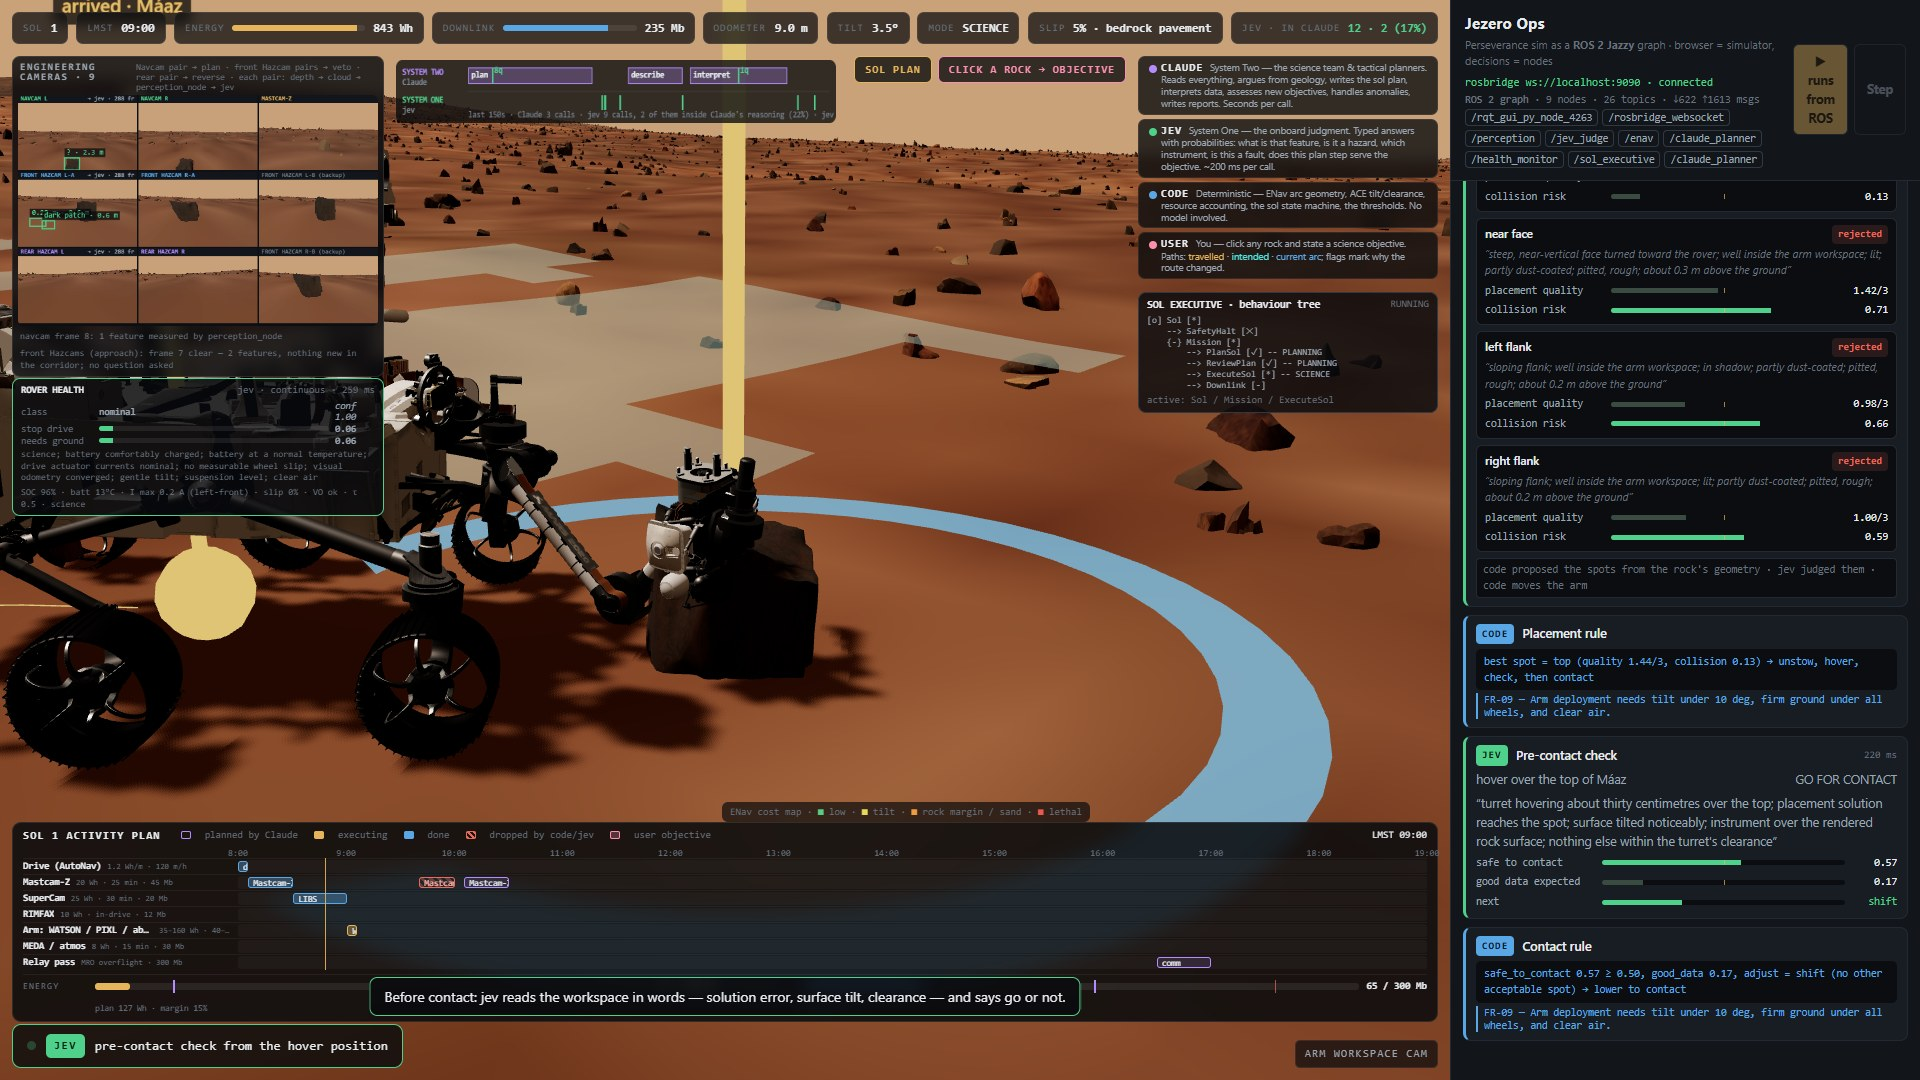
\includegraphics[width=\textwidth]{figs/arm-contact.jpg}
\caption{Arm placement at a science stop (recorded run). The arm workspace camera: the turret has been brought over the spot jev chose and lowered to contact after the pre-contact check. Console (right): the placement card --- four candidate spots with jev's quality score and collision risk, the chosen one marked --- the placement rule citing FR-09, the pre-contact card (safe to contact, good data expected, next) and the contact rule. Markers on the rock show the candidate spots: green chosen, grey acceptable, red rejected.}
\label{fig:arm}
\end{figure}

\paragraph{Real hardware.} \texttt{docs/hardware-contract.md} maps every simulator interface to the standard ROS\,2 interface a rover provides --- odometry and \texttt{tf2}, \texttt{BatteryState}/\texttt{Temperature}/\texttt{DiagnosticArray}, \texttt{stereo\_image\_proc} clouds per camera pair, Nav2 \texttt{FollowPath} or \texttt{ros2\_control} for the drive, \texttt{FollowJointTrajectory} for mast and arm --- and what stays identical: perception, the jev services and the health monitor (they read words code makes from those streams), ENav, the executive, the Claude actions. On a rover the TypeSafe endpoint becomes an onboard deployment behind the same service names; the ground actions stay on Earth with a real relay delay.

\begin{sidewaysfigure}[p]
\centering
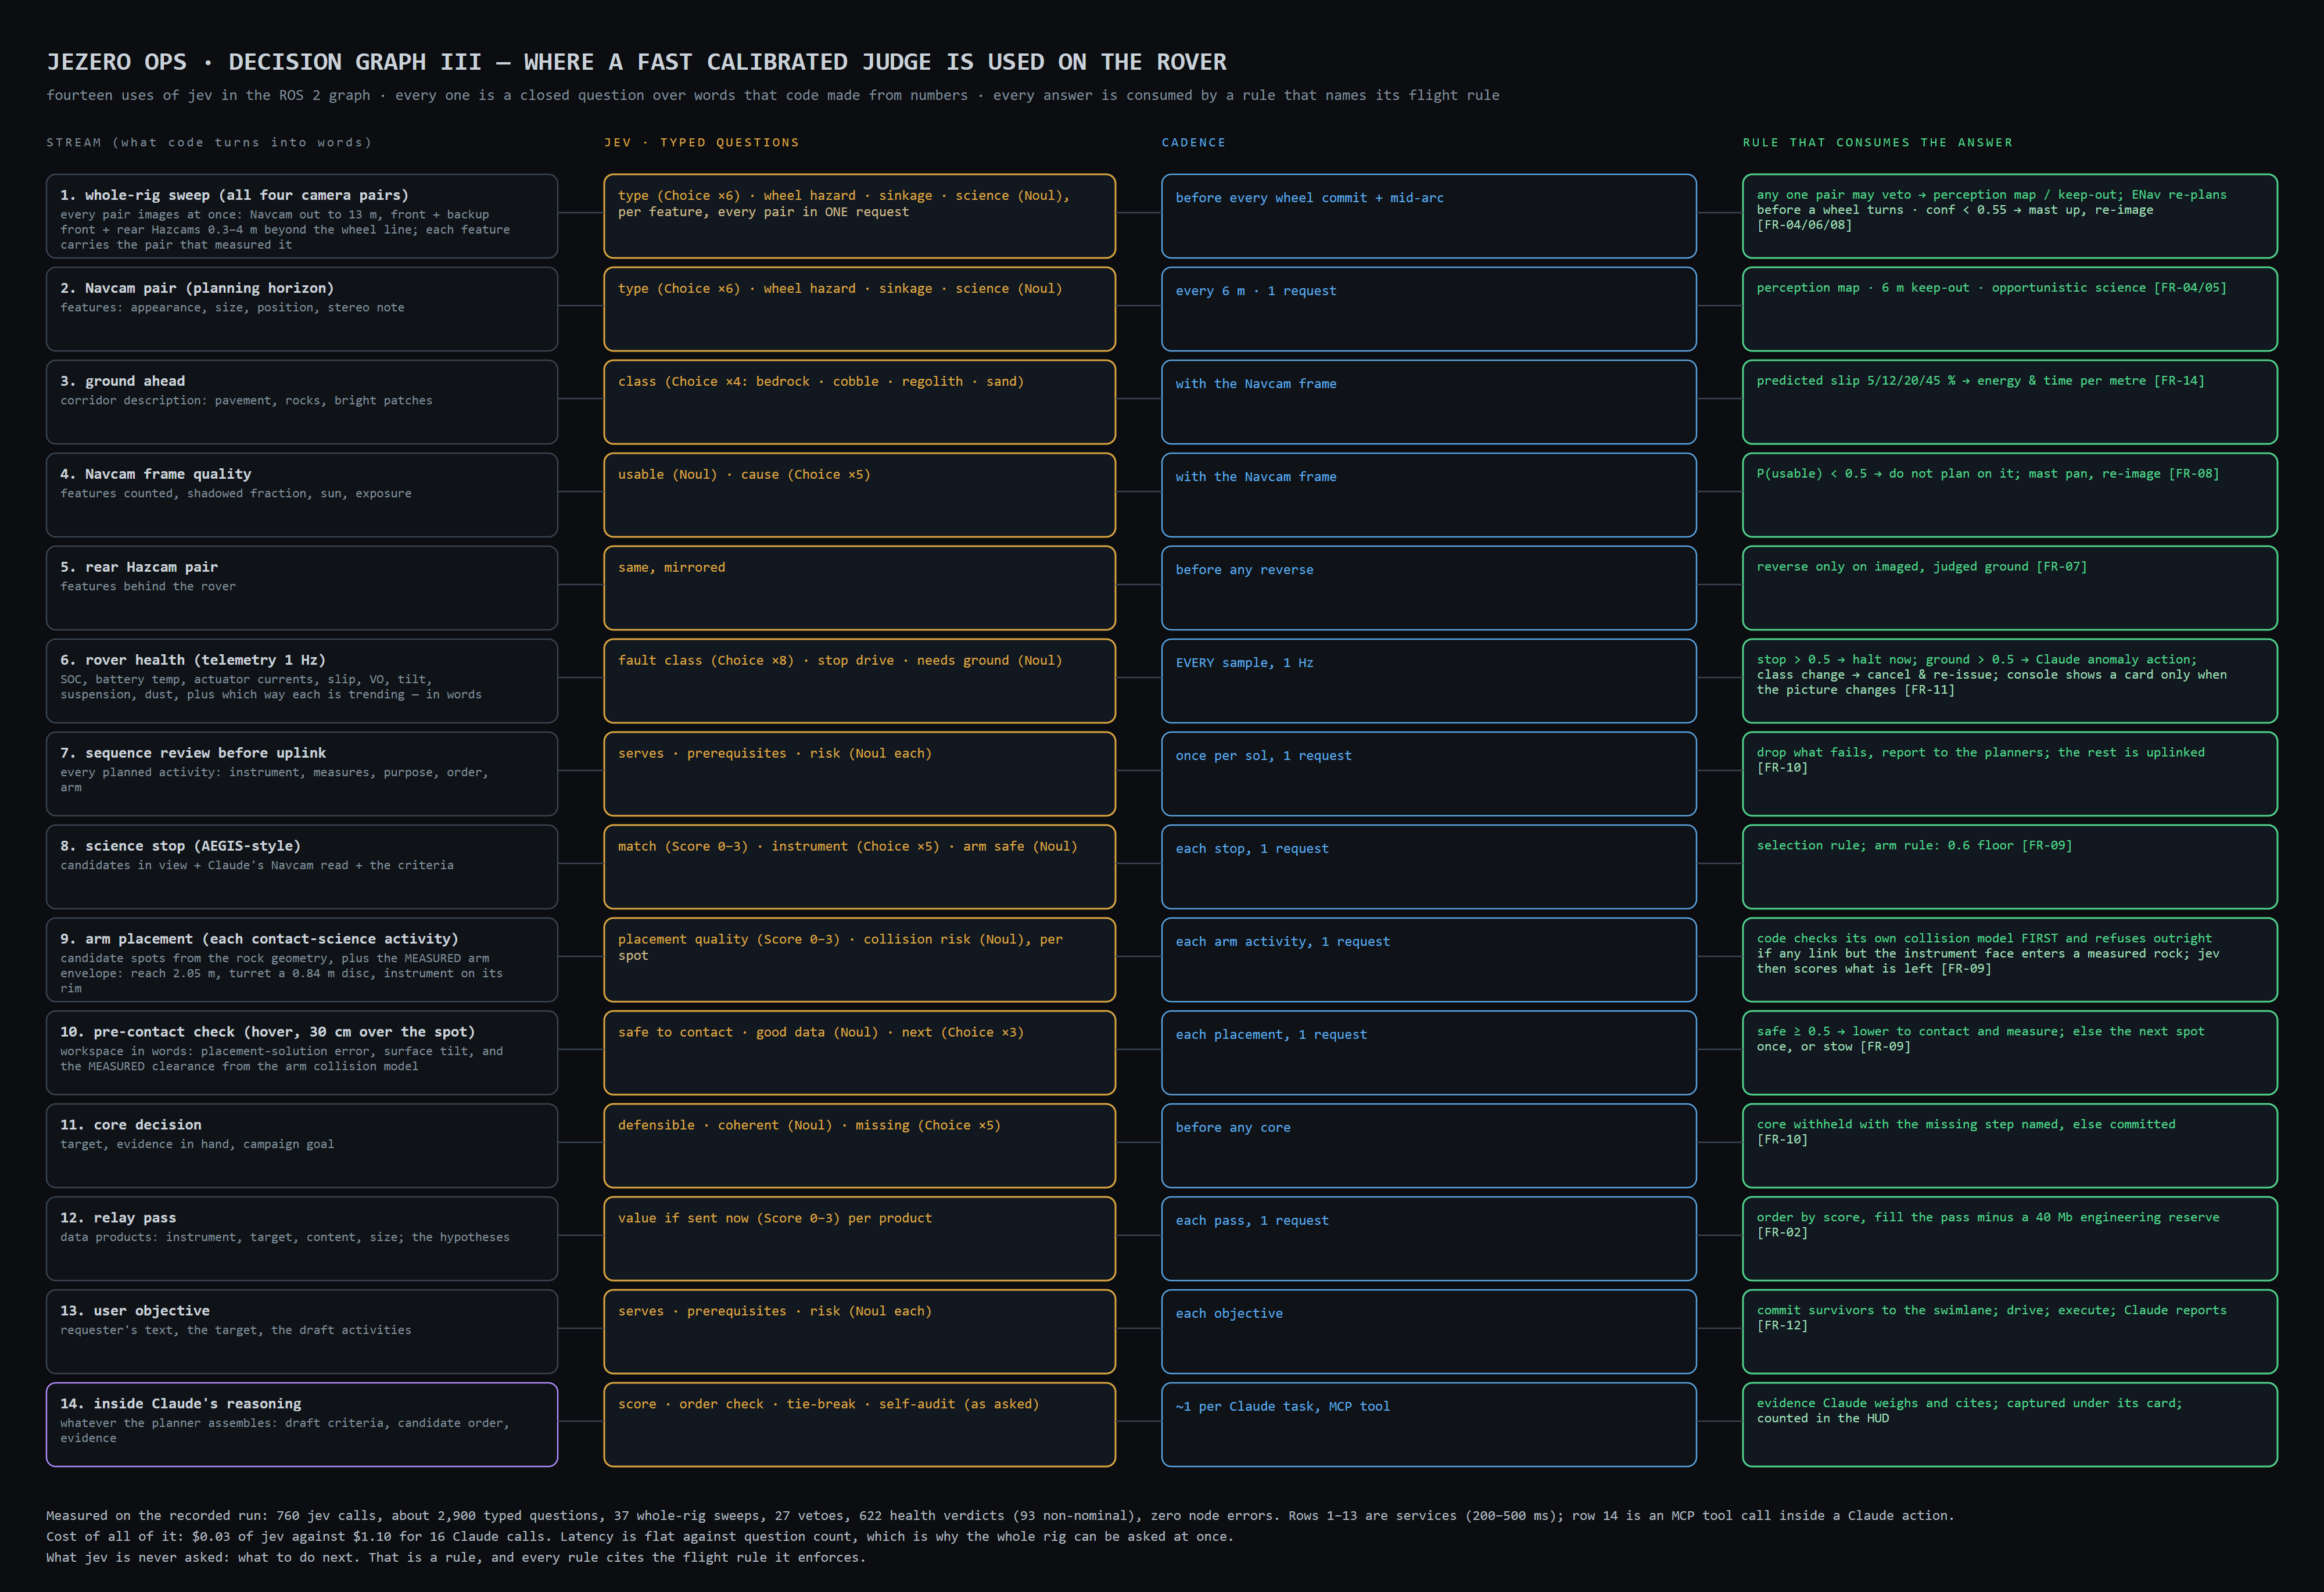
\includegraphics[width=\textwidth]{decision-graph-3.png}
\caption{Decision graph III: the fourteen places jev is used in the ROS\,2 graph --- the stream code turns into words, the typed questions, the cadence, and the rule (with its flight rule) that consumes the answer. Rows 1--13 are services; row 14 is the MCP tool inside a Claude action.}
\label{fig:graph3}
\end{sidewaysfigure}

\begin{figure}[p]
\centering
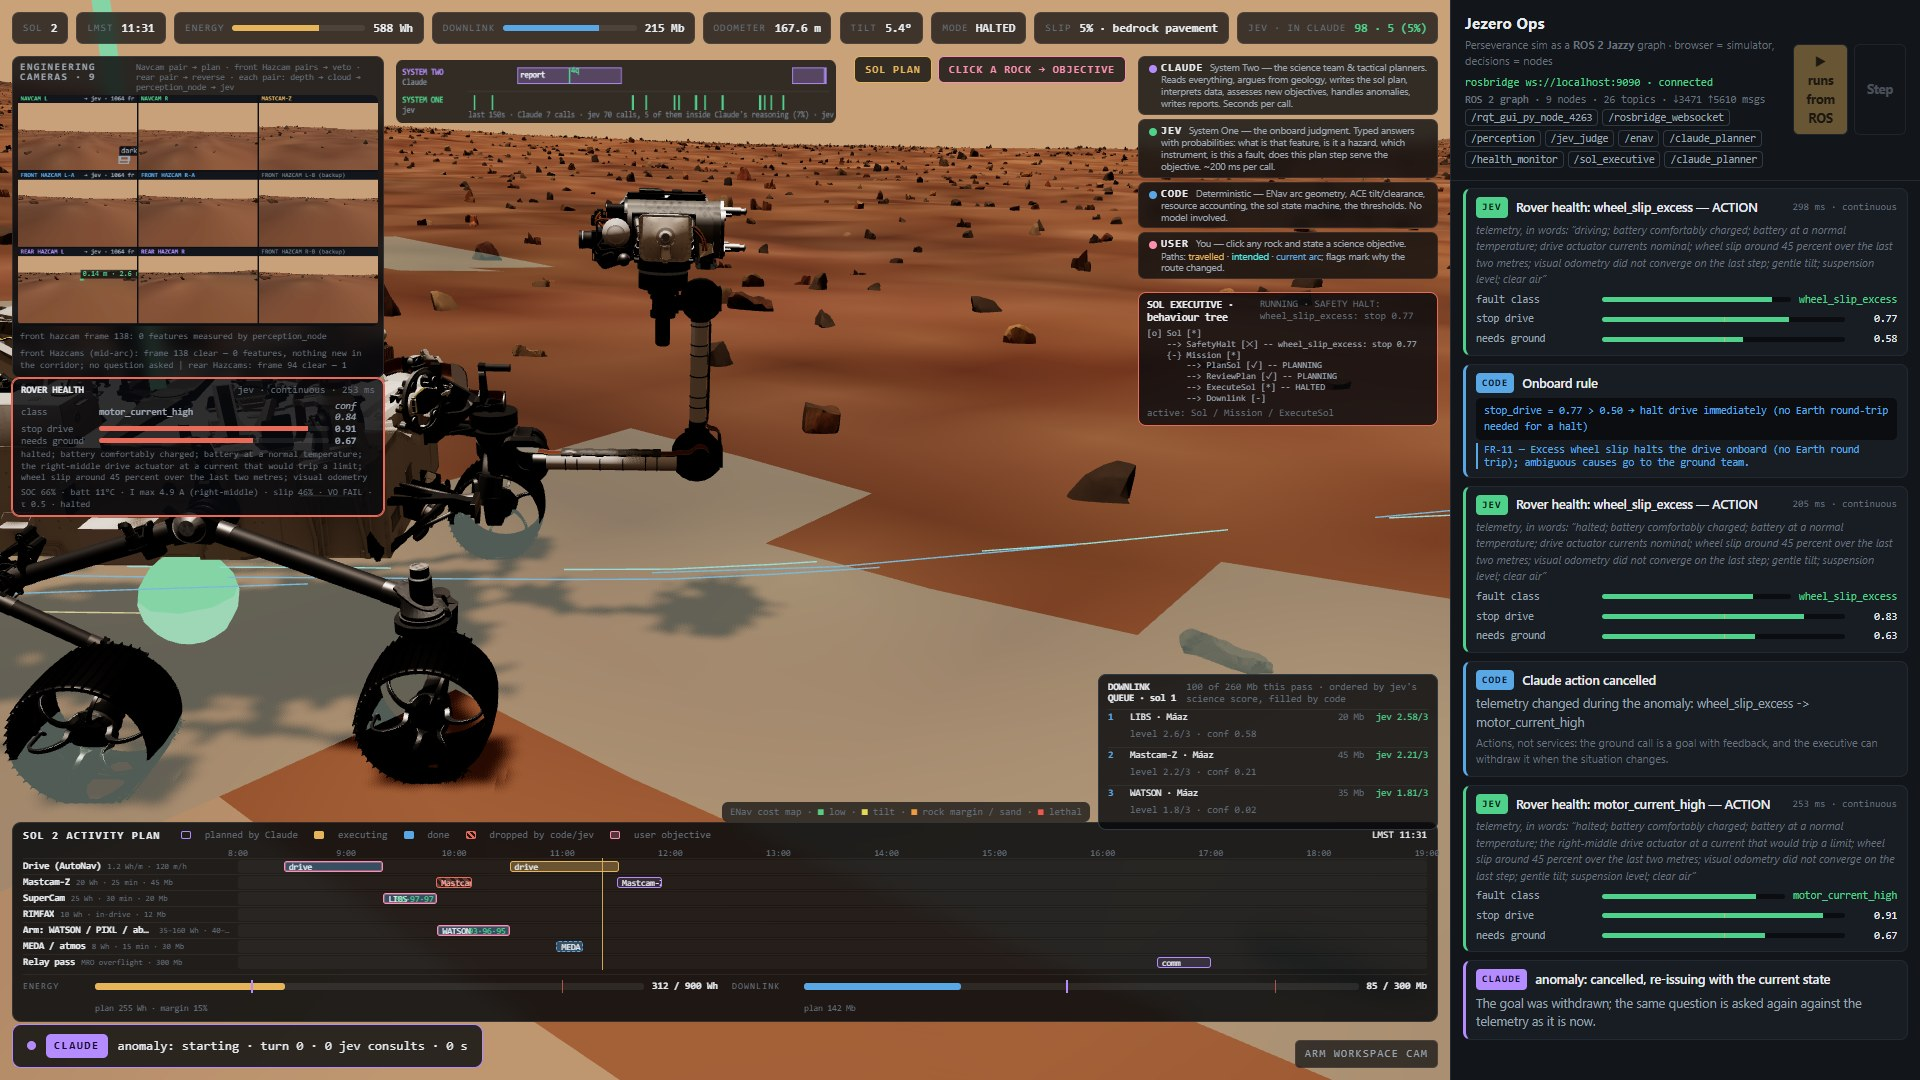
\includegraphics[width=\textwidth]{figs/flight-panels.jpg}
\caption{The page during the sol-2 health halt (odometer 168\,m, recorded run). Top right: the behaviour tree with the safety branch reporting the halt (\emph{wheel\_slip\_excess: stop 0.77}) while ExecuteSol stays the active leaf; top centre: the ``two speeds'' strip as the re-issued Claude anomaly action starts. Left: the rover-health panel --- jev's continuous verdict has moved from wheel slip to \emph{motor\_current\_high} (stop 0.91, ground 0.67) with the words it was shown and the raw housekeeping line beneath (4.9\,A on the right-middle actuator, slip 46\,\%, VO fail). Bottom right: the downlink queue from sol 1, ordered by jev's science score and filled by code. Console (right): the health card that halted the drive, the onboard rule citing FR-11, the verdict while halted, \emph{Claude action cancelled --- telemetry changed during the anomaly: wheel\_slip\_excess $\rightarrow$ motor\_current\_high}, and the re-issue. The overlays are sized so the rover stays visible in the middle.}
\label{fig:flight}
\end{figure}

\section{What each engine is trusted with}
\begin{itemize}
\item \textbf{Claude gets ambiguity, context, and language}: plans, interpretations, images, objectives, reports. Its outputs are constrained by JSON schemas so code can consume them, but the content is open-ended reasoning. It is slow and costs money; it runs a handful of times per sol.
\item \textbf{jev gets closed questions with defined answers}. It never sees the whole game state, only the fields a question needs. Its answers are probabilities, so every threshold is a line of code that can be inspected and tuned, and its confidence is a first-class signal that code routes on.
\item \textbf{Code gets everything that must be exact or repeatable}: arithmetic, geometry, resource accounting, ordering, margins, and the decision of when to ask which model. Neither model is ever asked ``what should happen next?''
\item \textbf{And Claude gets jev as a tool} --- the one place the two speeds touch directly. Claude decides what to ask; jev decides the answer; code records both and never lets an answer act on the rover except through Claude's structured output, which the onboard jev then verifies again.
\end{itemize}
The three colours on screen are the audit trail, not decoration. The green ticks inside the purple blocks are the newest part of it.

\section{What was done today}
\begin{enumerate}
\item Verified the TypeSafe skill and API (all three primitives, 0.4\,s), then built a small first game to learn the shape: eleven parallel questions per turn and a code-owned decision path rendered live.
\item Pulled the official assets --- USGS CTX DTM and orthomosaic, the NASA/JPL Perseverance model --- built the terrain from the real DEM with a Golombek rock field, and split the wheels in Blender.
\item Built the simulation: three.js world, ENav in code, jev question sets for hazards, target selection and faults, Claude prompts and schemas for planning, interpretation and anomalies, and an ops console showing every call's inputs and outputs.
\item Added, on request: the swimlane sol plan with per-instrument power, time and data; click-a-rock objectives with jev verification and Claude reports; travelled and intended path lines with reason flags.
\item Fixed what the takes revealed: a mounting error that had the rover driving backwards; an ENav deadlock when keep-outs surrounded the rover; rocks being driven over (a wheel-track and belly footprint replaced the circular one); flag clutter.
\item Replaced the rock-list ``perception'' with real perception: a rendered Navcam, depth-based blob measurement, sparse stereo in shadow, and Claude reading the frame at science stops.
\item Recorded the run with Playwright, encoded with Blender's sequencer, and uploaded to Drive by driving Chrome at the operating-system level after Chrome's own automation locks blocked every other route.
\item Moved the whole graph onto ROS\,2 Jazzy in a fresh WSL\,2 distro: \texttt{jezero\_msgs} (22 messages, 7 services), five nodes, the browser reduced to a simulator on rosbridge; a full three-sol run with the objective injection completed with no node errors.
\item Added the nine-camera engineering rig and the flight-like check cadence: every stereo pair produces its own cloud, the front Hazcams are asked before every segment and mid-arc, the rear pair before any reverse; reversing no longer reads the world's rock list.
\item Re-recorded the run on ROS\,2, replaced every screenshot in this report with one from that run, and wrote this report and the vision paper in Markdown and \LaTeX{} with PDFs.
\item Fifth pass (goal 4): the robotic arm became a real kinematic chain driven by inverse kinematics; jev scores the candidate placement spots code derives from the rock geometry and clears contact from the hover position; photogrammetry rocks; re-recorded and rewritten.
\item Fourth pass (goal 3): Claude calls became ROS\,2 actions with feedback and cancel; the executive became a \texttt{py\_trees} behaviour tree with a safety branch; a health-monitor node runs jev on the 1\,Hz telemetry stream; jev added to sequence review before uplink, frame usability, sample defensibility and downlink prioritisation; a hardware contract mapping every simulator interface to its standard ROS\,2 equivalent; re-recorded and rewritten.
\item Third pass (goal 2): gave Claude jev as an MCP tool while it reasons, captured every consultation, and measured how much System One runs inside System Two; added flight-rule citations on every gate, slip prediction by terrain class, the ENav cost map, camera frusta and the two-speeds strip; drew Decision Graph II; re-recorded and rewrote the papers and the ROS\,2 notes.
\end{enumerate}

\section{ROS\,2}
\label{sec:ros2}
The same graph now runs as a ROS\,2 Jazzy system (Ubuntu 24.04 under WSL\,2). The browser keeps only what a simulator owns --- terrain, the rover's motion, the camera rig, rendering, the HUD --- and talks to the graph over rosbridge; perception, jev judgment, ENav, the LLM planner and the sol executive are nodes with typed interfaces (\texttt{jezero\_msgs}: 22 messages, 7 services; Figure~\ref{fig:rosgraph}). Every decision is a \texttt{Decision} message carrying its engine, so a bag replays the attribution stream. A full three-sol run --- plans, the perception loop, science stops with Claude reading the Navcam frame, a user objective verified by jev and reported by Claude, and Claude consulting jev while it reasons --- completed over the graph with no node errors and is recorded as \texttt{jezero-ops-ros2-v2-1080p.mp4}.

The port is also where Section~\ref{sec:cameras} became real (Figure~\ref{fig:rig}): the simulator renders the nine engineering cameras, each stereo pair produces its own point cloud, and the executive's drive loop asks jev about the Navcam pair every 6\,m, and puts the \emph{whole rig} --- all four camera pairs at once --- to jev before any wheel is committed and again mid-arc, with the rear pair before any reverse. jev is asked only about features that are new, inside the wheel corridor, and not already cleared by geometry; a \emph{veto} puts the rock into the perception map and ENav re-plans before a wheel moves. In the recorded three-sol run (22 minutes) that was 37 whole-rig sweeps and 27 vetoes, 622 health verdicts at 1\,Hz of which 93 were non-nominal, 760 jev calls carrying about 2\,900 typed questions, and 13 Claude calls (\$1.10 against \$0.03 of jev), with no node errors. Reversing no longer reads the world's rock list: the rear Hazcams see for themselves. \texttt{docs/ros2-migration.md} has the node table, the run recipe and what is still a simulator shortcut.

\begin{figure}[p]
\centering
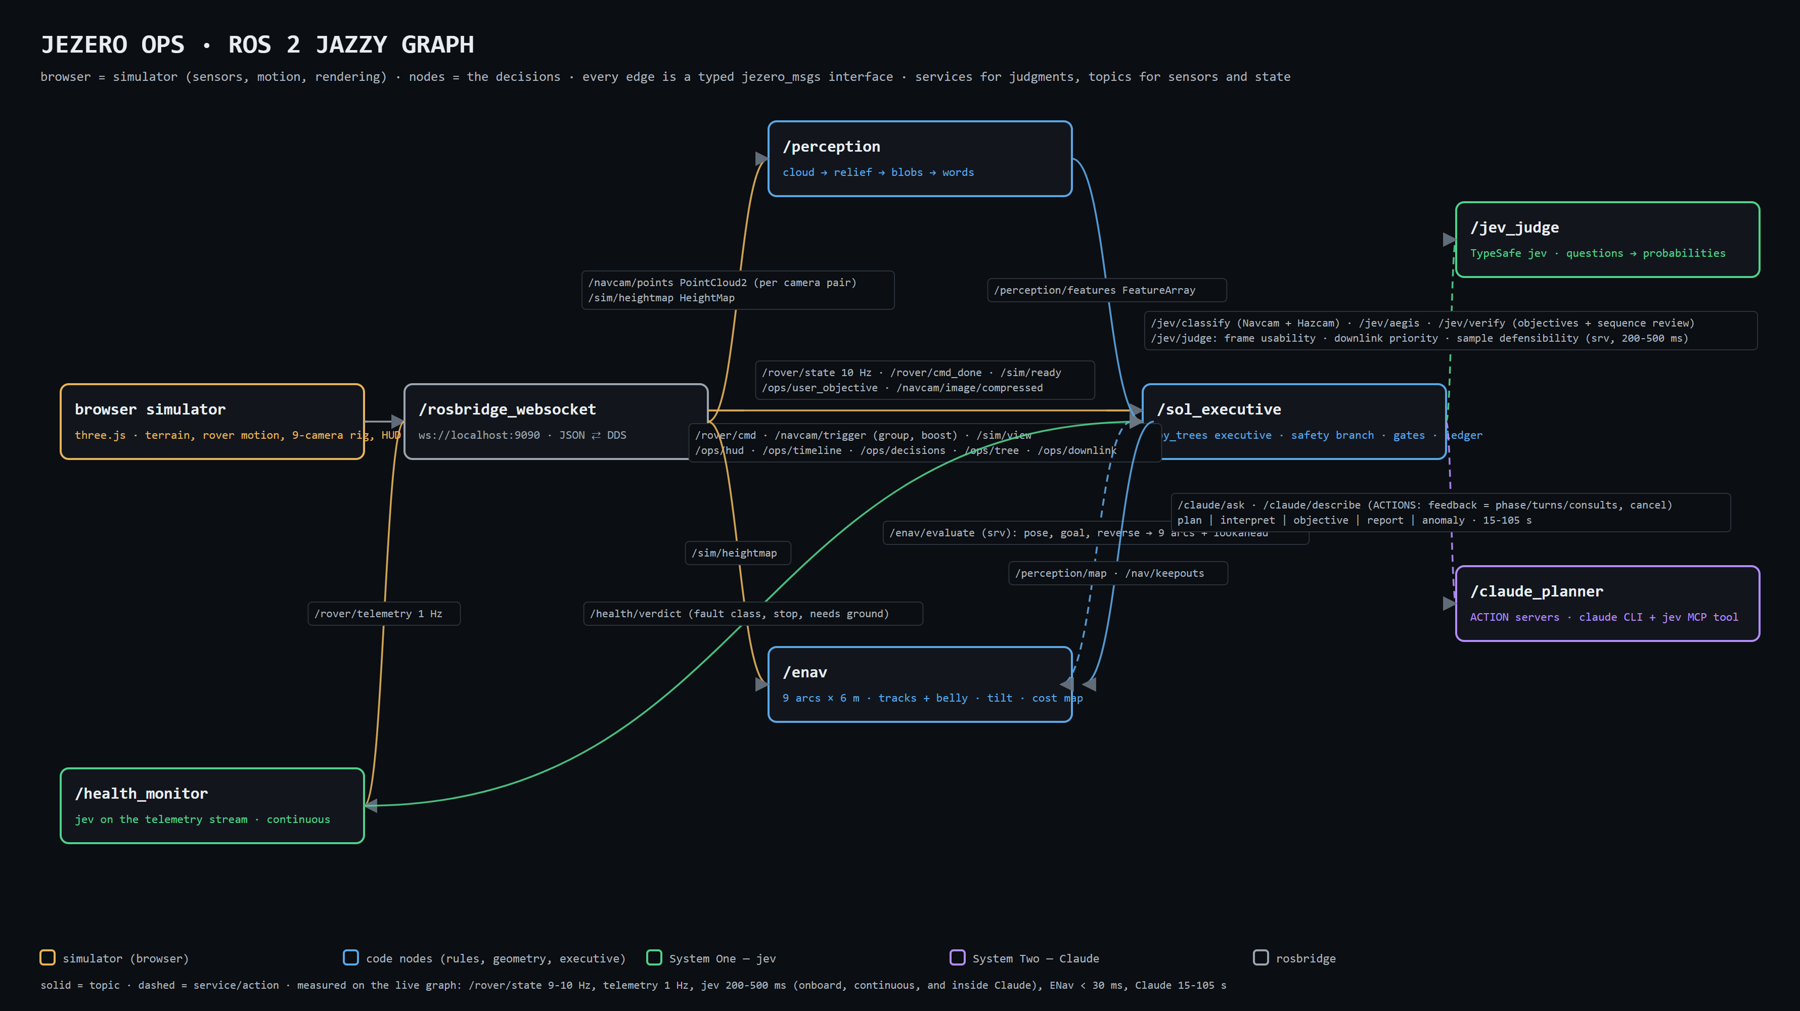
\includegraphics[width=\textwidth]{figs/ros2-graph.png}
\caption{The live ROS\,2 graph. Gold: the browser simulator (sensors, motion, rendering). Blue: code nodes --- perception, ENav, the sol executive. Green: jev behind four services. Purple: Claude behind two. Solid edges are topics, dashed are services; measured on the running graph, \texttt{/rover/state} at 9--10\,Hz, jev 200--300\,ms, ENav under 30\,ms, Claude 15--80\,s.}
\label{fig:rosgraph}
\end{figure}

\begin{figure}[p]
\centering
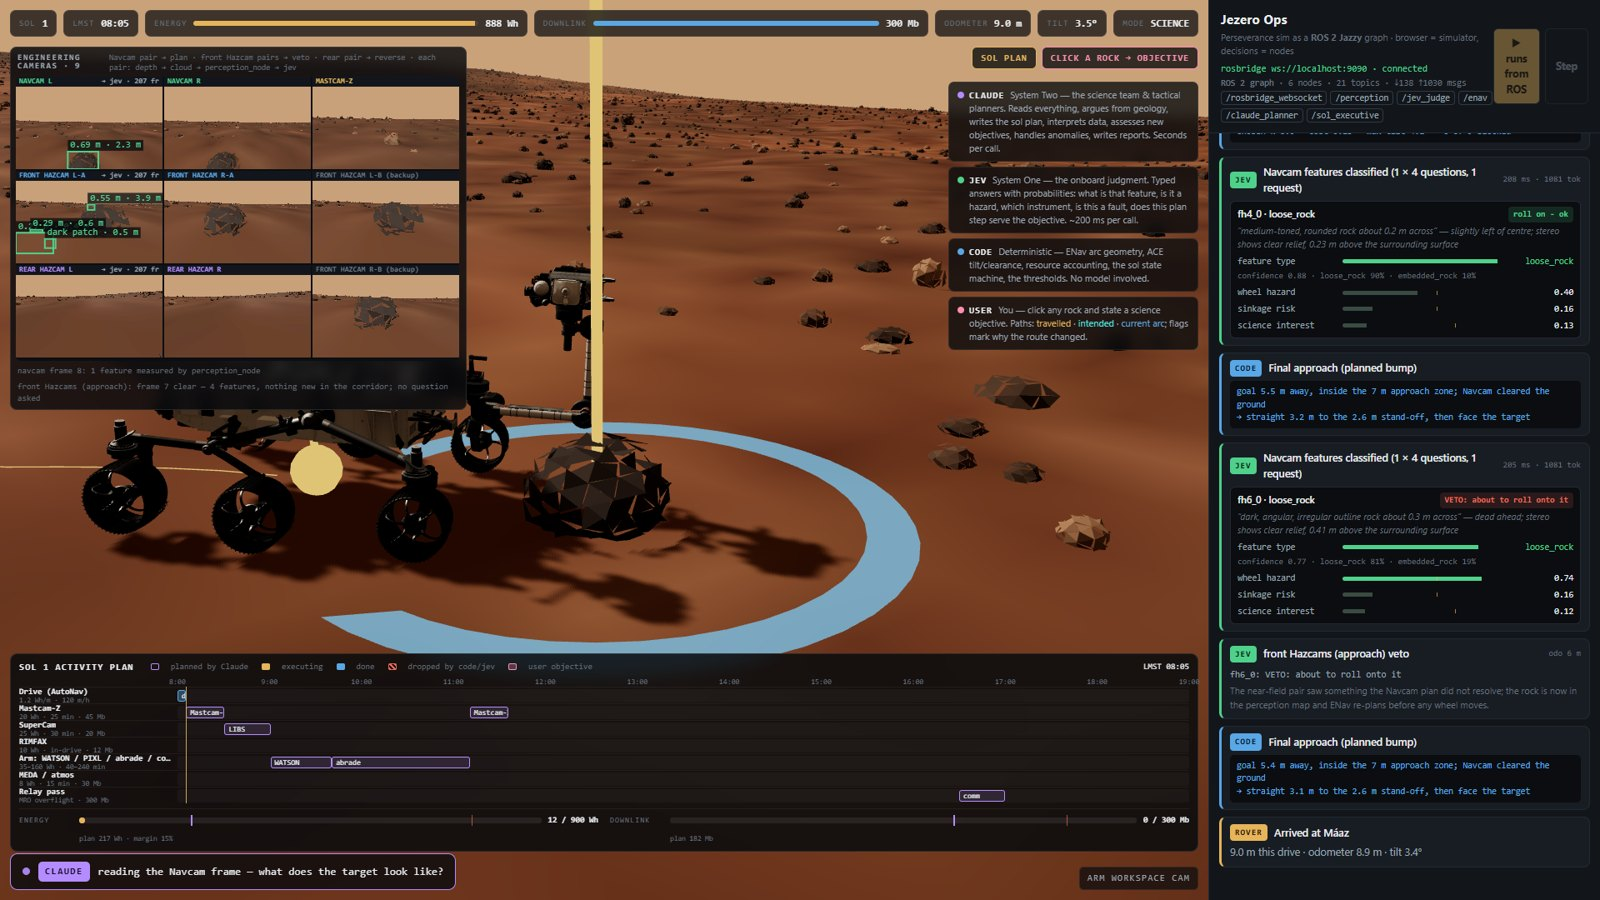
\includegraphics[width=\textwidth]{figs/ros2-rig.jpg}
\caption{The ROS\,2 page at the sol-1 science stop. Top left: the 3$\times$3 engineering-camera rig --- Navcam L/R and Mastcam-Z, front Hazcam pairs A and B, rear Hazcam L/R --- with perception's boxes on the primary camera of each pair and a status line per group (``front Hazcams (approach): frame 7 clear --- 4 features, nothing new in the corridor; no question asked''). Top right: the live graph panel (6 nodes, 21 topics, message counters). Console: a front-Hazcam jev card that vetoed the approach (\emph{about to roll onto it}, $P=0.74$), the executive's planned bump to the stand-off, and arrival.}
\label{fig:rig}
\end{figure}

\section{Measuring instead of asserting}
Every earlier pass of this report described what the system \emph{does}. This one describes what it \emph{achieves}, because the qualitative claims turned out to be hiding two real defects. Each number below comes from a tool in \texttt{tools/} that scores the system against the world's rock list --- ground truth the rover itself never reads.

\subsection{Perception: a shadow model that ate its own boulders}
Stereo fails in deep shadow, and the pipeline modelled that by discarding shadowed pixels at random. Randomly deleting 65\,\% of a region's pixels destroys 4-connectivity: a shadowed boulder came apart into single-pixel fragments, every one of them under the blob floor, and the only thing left that still joined up was the flat dark skirt around its base. The rock was therefore reported as \texttt{dark\_patch} --- \emph{a shadow}. For a driver that is the worst available error, and it was invisible because every individual stage looked correct.

Real stereo does not fail pixel by pixel. A correlation window either finds a match or it does not, and neighbouring windows fail together. Dropout is now applied on a $4\times4$ block hash; components are 8-connected; and thresholding is hysteresis, seeding on relief above 0.075\,m and growing into relief above 0.028\,m so the box is the rock's whole footprint rather than its crown. Perception renders at $384\times216$ rather than $192\times108$.

\begin{center}
\begin{tabular}{@{}lrr@{}}
\toprule
& before & after \\
\midrule
recall, all rocks $\geq$ 0.35\,m & 3.6\,\% & \textbf{13.9\,\%} \\
recall, 0.5--0.8\,m & 8\,\% & \textbf{20\,\%} \\
recall, 0.8--1.2\,m & 33\,\% & \textbf{56\,\%} \\
ten largest rocks at 4\,m stand-off & 3/8 & \textbf{8/8} \\
median size error & 57\,\% & \textbf{47\,\%} \\
\bottomrule
\end{tabular}
\end{center}

The remaining gap is range, not logic. \texttt{traverse\_eval} walks a forced straight line with ENav switched off and counts rocks above the 0.20\,m step limit that end up under a wheel: six in 60\,m, of which the perception map held two and had never seen the other four. So the rover drives over roughly ten step-limit rocks per 100\,m, and most of those it never saw. That is a perception budget problem --- a denser stereo pipeline and a higher imaging cadence --- not a property of the decision graph.

\subsection{The arm: a turret seven times bigger than its collision model}
The second defect was visible in a single frame: the turret buried inside a boulder while the console reported clearance. The collision model approximated the turret as a capsule of radius 0.12\,m. Measured off the model, the turret is a disc $0.83\times0.34\times0.84$\,m, and the instrument sits on its \emph{rim}, 0.37\,m from the turret's own pivot. The model was wrong by a factor of seven in the one dimension that mattered.

Nothing is approximated now. Points are sampled off the turret's real meshes and transformed by the live pose; the long links stay capsules, which they genuinely are; and only geometry within 0.10\,m of the instrument face is allowed inside a rock, because that is the part whose job is to touch. Rocks became ellipsoids sized to the measured footprint and relief --- a sphere sized to a wide flat slab's footprint stands a metre taller than the slab does, and that phantom height was rejecting exactly the placement a rover wants, the instrument flat on the top facet.

That done, the stand-off distance turned out to be wrong too, and the measurement said so:

\begin{center}
\begin{tabular}{@{}lrrr@{}}
\toprule
stand-off & accepted & top-facet & accepted but penetrating \\
\midrule
1.2\,m & 1/24 & 1/10 & 0 \\
\textbf{1.6\,m} & \textbf{20/30} & \textbf{10/10} & \textbf{0} \\
2.0\,m & 9/30 & 1/10 & 0 \\
2.3\,m (the old value) & 10/30 & 0/10 & 0 \\
\bottomrule
\end{tabular}
\end{center}

At 2.3\,m the arm has to stretch out nearly flat over the rock to reach its top, and the forearm grazes it; at 1.2\,m the rock is under the front wheels and inside the folded arm. FR-13 now commands a 1.6\,m stand-off, derived from the measured envelope rather than chosen. Across every configuration the number of accepted placements that penetrate the rock is zero --- and about two thirds of candidate spots are now refused, which is the honest consequence of a turret that wide. The measured envelope is also given to jev, in \texttt{arm\_envelope}. Before that, jev was scoring placements without knowing the size of the thing it was placing.

\subsection{What the cameras can see, drawn on the ground}
Each camera's depth frame is splatted into a world-space coverage map. The occlusion is exact by construction rather than by a shadow test, because the splat \emph{is} what the depth buffer recorded: the ground behind a rock was never measured, so it is never marked. Parking the rover 7\,m from each of the ten largest rocks in the area and sampling the map inside the geometric shadow and beside it at the same range gives mean coverage behind a rock 0.10, beside it 0.87, with nine of ten casting a proper shadow.

One instructive failure along the way: an early version stretched each splat along the view ray to hide striping in the far field. A splat from a rock's \emph{top} surface then spilled past the rock and painted the ground behind it, filling in the occlusion shadow the map exists to show. The striping is the honest artefact; the smoothing was the lie.

\begin{figure}[h]
\centering
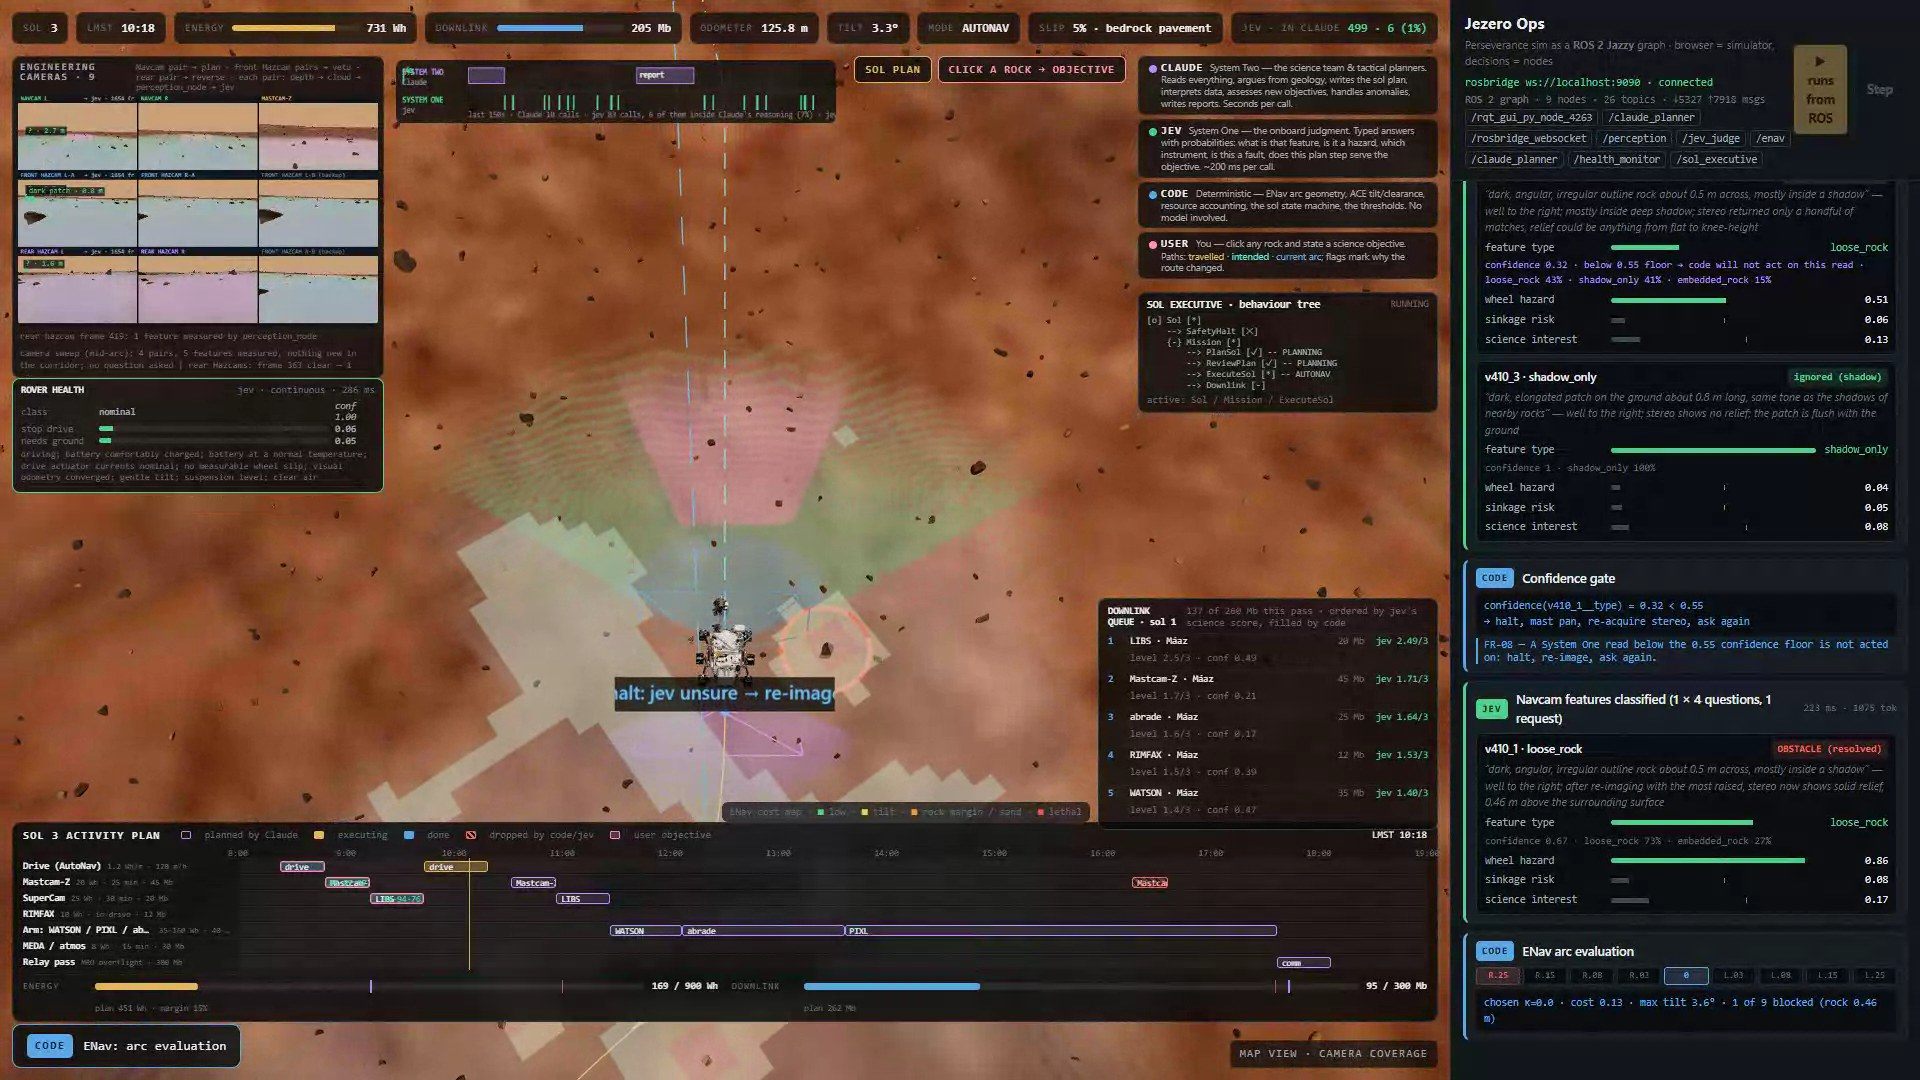
\includegraphics[width=\textwidth]{figs/coverage-map.jpg}
\caption{The coverage map, mid-drive. Each camera group paints in its own colour: green Navcam out to 20\,m, blue front Hazcams in the near field, violet rear, magenta Mastcam-Z. Pale ground behind the rover is everywhere the rig has held a clear line. The console shows a confidence gate resolving: jev returned \texttt{shadow\_only} at 0.32, below the 0.55 floor, so code refused to act, raised the mast and re-imaged; the second look came back \texttt{loose\_rock} at 0.67 with 0.46\,m of measured relief, and the rock went into the perception map.}
\label{fig:coverage}
\end{figure}

\subsection{jev at a cadence an LLM could not reach}
Before any wheel is committed, and again mid-arc, every camera pair images and everything new in the corridor goes to jev in one request; one veto from any pair stops the move. And jev now reads every telemetry sample, roughly one a second, with trend terms so a channel on its way somewhere is caught before it trips a limit.

The recorded run: 37 whole-rig sweeps, 27 vetoes, 622 health verdicts of which 93 non-nominal, 760 jev calls and about 2\,900 typed questions in total. Measured cost: \$0.03 of jev against \$1.10 of Claude, which is the whole argument in two numbers. Latency is flat against question count --- a request carrying 48 questions returns in the same ${\sim}250$\,ms as one carrying 4 --- so batching the whole rig costs nothing in time either.

A caution that came out of this: the framing of a question moves the answer. When the sweep described a feature nine metres away as ``under the next wheel placement'', jev's confidence fell to 0.28--0.56 and the 0.55 gate halted the rover on nearly every sweep. The words a System One model is given have to match the measurement; a state that quietly misdescribes the world produces a model that is correctly uncertain about a question nobody meant to ask.

\subsection{A twenty-minute run as a two-minute video}
Roughly two thirds of a run's wall clock is Claude reasoning with nothing moving. The CLI itself adds only about 1.2\,s per call, and jev about 250\,ms, so there is no idle time to remove --- the model is genuinely thinking. The run is therefore not made shorter; the recording is re-timed. A speed plan derived from the run's own event log keeps the moments where a decision changes something at real time and compresses the rest, with the multiplier burned into the corner throughout. The recorded run: 1\,333\,s of wall clock, 120\,s of video, 14 real-time windows.

\section{Honest limits}
This is a demonstration. It is not flight software, it has not been validated against rover data, and the numbers above describe a simulator scoring itself against its own ground truth.

\begin{itemize}
\item \textbf{Small rocks are missed and driven over}: 7\,\% recall at 0.35--0.5\,m, 20\,\% at 0.5--0.8\,m, and about ten step-limit rocks per 100\,m ending up under a wheel, most of them never perceived.
\item \textbf{Two thirds of arm placements are refused} because the turret is 0.84\,m across and reaches 2.05\,m. The refusals are correct; the workspace is simply small.
\item The arm's collision model is sampled points and capsules against ellipsoids. Much better than a guess, and still not the real turret mesh against the real rock mesh.
\item The back-up-and-drive-around manoeuvre exists and fires when every forward arc is blocked, but it is rare enough in a recorded run to be easy to miss. The demo does not showcase it well.
\item Instrument results are one-paragraph summaries from a truth table, not spectra.
\item The dust devil and slip event are scripted so they reliably appear in a short run; sand, rocks and shadows are perceived.
\item Perception uses the renderer's depth buffer as an idealised stereo stand-in with deliberate patch-wise dropout in shadow; real stereo is noisier everywhere.
\item jev's calibration is taken from its documentation and spot checks, not rover data.
\item Claude's tactical plans are sound geology but sometimes over-plan a sol; the scheduler drops what does not fit.
\end{itemize}

None of these is a limit of the architecture. They are a perception pipeline that needs to be denser, a turret that needs a real collision mesh, and a demo that needs more takes.

\begin{thebibliography}{9}
\bibitem{fergason} R.\,L. Fergason, T.\,M. Hare, D.\,P. Mayer et al., ``Mars 2020 Terrain Relative Navigation Flight Product Generation: Digital Terrain Model and Orthorectified Image Mosaics,'' LPSC 51, 2020. \href{https://doi.org/10.5066/P906QQT8}{doi:10.5066/P906QQT8}.
\bibitem{nasa3d} NASA/JPL-Caltech, \emph{Mars Perseverance Rover 3D model}, science.nasa.gov.
\bibitem{golombek} M.\,P. Golombek et al., rock size--frequency distributions at Mars landing sites (cumulative fractional area model).
\bibitem{polyhaven} Poly Haven, CC0 photogrammetry rock scans (moon\_rock\_01--07, namaqualand\_boulder\_02/03/05/06, namaqualand\_stones\_01, rock\_09, stone\_01), \url{https://polyhaven.com}.
\bibitem{enav} JPL, ``NASA's Self-Driving Perseverance Mars Rover `Takes the Wheel'\,'' (AutoNav, $\sim$120\,m/h); M. Ono et al., ENav and Approximate Clearance Evaluation, arXiv:2011.06022.
\bibitem{jplplanning} JPL AI Group, ``Onboard Planning for the Mars 2020 Perseverance Rover,'' ASTRA 2022; ``Evolution of the Mars 2020 Perseverance Rover's Strategic Planning Process.''
\bibitem{maki} J.\,N. Maki et al., ``The Mars 2020 Engineering Cameras and Microphone on the Perseverance Rover,'' \emph{Space Science Reviews} 216, 137 (2020). Navcam, Hazcam and CacheCam fields of view and placement.
\bibitem{typesafe} TypeSafe documentation: \emph{How to build with TypeSafe}, \emph{Primitives}, \emph{Confidence}, \emph{Jev 1.13 jaggedness}. \url{https://docs.typesafe.ai}.
\end{thebibliography}
\end{document}
